\documentclass[conference]{IEEEtran}
\IEEEoverridecommandlockouts
% The preceding line is only needed to identify funding in the first footnote. If that is unneeded, please comment it out.
\usepackage{cite}
\usepackage{amsmath,amssymb,amsfonts}
\usepackage{algorithmic}
\usepackage{graphicx}
\usepackage{textcomp}
\usepackage{xcolor}
\usepackage[utf8]{inputenc}
\usepackage[vietnamese]{babel}
\usepackage{amsmath}
\usepackage[table]{xcolor}

\def\BibTeX{{\rm B\kern-.05em{\sc i\kern-.025em b}\kern-.08em
    T\kern-.1667em\lower.7ex\hbox{E}\kern-.125emX}}
\begin{document}

\title{Dự báo chất lượng không khí tại Việt Nam bằng phương pháp chuỗi thời gian\\
{\footnotesize \textsuperscript{}}
\thanks{Identify applicable funding agency here. If none, delete this.}
}

\author{
\IEEEauthorblockN{1\textsuperscript{st} Huỳnh Lê Phong}
\IEEEauthorblockA{\textit{Khoa Hệ thống thông tin}\\
\textit{Trường Đại học Công nghệ Thông tin}\\
21520086@gm.uit.edu.vn}
\and
\IEEEauthorblockN{2\textsuperscript{nd} Nguyễn Quốc Trạng}
\IEEEauthorblockA{\textit{Khoa Hệ thống thông tin} \\
\textit{Trường Đại học Công nghệ Thông tin}\\
21521556@gm.uit.edu.vn}
\and
\IEEEauthorblockN{3\textsuperscript{rd} Nguyễn Triệu Vy}
\IEEEauthorblockA{\textit{Khoa Hệ thống thông tin}\\
\textit{Trường Đại học Công nghệ Thông tin}\\
21522812@gm.uit.edu.vn}
\and
\IEEEauthorblockN{\hspace{4cm}4\textsuperscript{th} Vũ Thị Phương Linh}
\IEEEauthorblockA{\hspace{3.6cm}\textit{Khoa Hệ thống thông tin}\\
\hspace{3.6cm}\textit{Trường Đại học Công nghệ Thông tin}\\
\hspace{3.6cm}20521541@gm.uit.edu.vn}
\and
\IEEEauthorblockN{\hspace{-2cm}5\textsuperscript{th} Đỗ Đình Đăng Khoa}
\IEEEauthorblockA{\hspace{-2.4cm}\textit{Khoa Hệ thống thông tin}\\
\hspace{-2.4cm}\textit{Trường Đại học Công nghệ Thông tin}\\
\hspace{-2.4cm}21522218@gm.uit.edu.vn}

}


\maketitle

\begin{abstract}
Nghiên cứu này tập trung vào phân tích chất lượng không khí ở ba thành phố lớn tại Việt Nam: Hà Nội, Hạ Long và Việt Trì. Mục tiêu của nghiên cứu là sử dụng các kỹ thuật phân tích chuỗi thời gian tiên tiến để dự báo và hiểu các chỉ số chất lượng không khí như PM2.5, PM10, O3, NO2, SO2 và CO. Phương pháp phân tích bao gồm cả các thuật toán truyền thống và tiên tiến như Hồi quy Tuyến tính, Mô hình ARIMA, Mạng Nơ-ron Hồi quy (RNN), Đơn vị Hồi quy Cổng (GRU), LSTM, VAR, Rừng Ngẫu nhiên, Mô hình Mã hóa Dày Chuỗi Thời gian (TiDE), Autoformer, Mạng Nơ-ron Đa Tầng (MLP). Chúng tôi sử dụng hai tỷ lệ khác nhau giữa các tập dữ liệu huấn luyện: testing, cụ thể là 7:3, 8:2 và 9:1, để đánh giá hiệu suất của các mô hình dưới các điều kiện khác nhau. Sau đó, nó so sánh hiệu suất của các mô hình khác nhau dựa trên ba chỉ số: Mean Absolute Percentage Error (MAPE), Root Mean Square Error (RMSE), và Mean Logarithmic Square Error (MLSE). Cuối cùng, hai mô hình có hiệu suất tốt nhất được sử dụng để dự báo chất lượng không khí cho 30 ngày tiếp theo, thể hiện hiệu quả của chúng trong việc dự báo chất lượng không khí. Bằng cách sử dụng các tập dữ liệu thời gian thực, nghiên cứu này nhằm dự báo, khám phá các mẫu, xu hướng và mối quan hệ giữa các chỉ số chất lượng không khí. Ngoài ra, nghiên cứu cũng nhằm đóng góp vào việc hiểu rõ hơn về việc giải quyết các vấn đề ô nhiễm không khí, thúc đẩy môi trường đô thị khỏe mạnh và bền vững hơn.
\end{abstract}

\begin{IEEEkeywords}
Chất lượng không khí, ô nhiễm không khí, phân tích chuỗi thời gian, dự báo, Hồi quy Tuyến tính, ARIMA, RNN, GRU, LSTM, VAR, Random Forest, TiDE, Autoformer, MLP, Hà Nội, Hạ Long, Việt Trì, Việt Nam.
\end{IEEEkeywords}

\section{Giới thiệu}
\section{Nghiên cứu liên quan}

Trong những năm gần đây, đã có một sự gia tăng đáng kể trong nghiên cứu nhằm dự báo chất lượng không khí bằng cách sử dụng một loạt các kỹ thuật máy học, học sâu và thống kê.

Evgeniy Marinov, Dessislava Petrova-Antonova và Simeon Malinov, trong một nghiên cứu \cite{b1}, tập trung vào việc cải thiện độ chính xác của việc dự báo chất lượng không khí thông qua việc áp dụng phương pháp ARIMA. Nghiên cứu của họ, dựa trên dữ liệu từ các trạm giám sát chất lượng không khí tại Thành phố Sofia, Bulgaria, từ ngày 1 tháng 1 năm 2015 đến ngày 31 tháng 12 năm 2019, đã cho thấy hiệu quả của các mô hình ARIMA trong việc dự báo nồng độ ô nhiễm như CO, NO2, O3 và PM2.5.

S. H. Khaerun Nisa, Irfan Irfani và Utriweni Mukhaiyar, trong nghiên cứu của họ \cite{b2}, đã khám phá việc dự báo mức độ ô nhiễm không khí tại Jakarta bằng phương pháp phân tích Vector Autoregressive (VAR). Bằng cách phân tích dữ liệu chuỗi thời gian về chỉ số chất lượng không khí (AQI) và nồng độ PM2.5 thu thập từ ngày 16 tháng 8 đến ngày 25 tháng 9 năm 2023, để huấn luyện, và từ ngày 25 tháng 9 đến ngày 1 tháng 10 năm 2023, để kiểm tra, họ đã xác định mô hình VAR(2) tối ưu cho việc dự báo ô nhiễm không khí chính xác.

Khawaja Hassan Waseem và cộng sự đã khám phá tác động của các yếu tố khí hậu đối với nồng độ PM2.5 và phát triển mô hình dự báo trong một nghiên cứu gần đây \cite{b3}. Nghiên cứu của họ, kéo dài trong 30 ngày và 72 giờ cho các dự đoán hàng ngày và hàng giờ tương ứng, đã kết hợp dữ liệu chất lượng không khí, chất gây ô nhiễm và điều kiện khí hậu từ nhiều thành phố ở Pakistan. Sử dụng các mô hình máy học và học sâu bao gồm FbProphet và LSTM, họ đã phát hiện mô hình mã hóa-giải mã LSTM vượt trội so với các mô hình khác, đạt được cải thiện đáng kể về độ chính xác dự báo.

Hai tác giả, Marwa Winis Misbah Esager và Kamil Demirberk Ünlü \cite{b4}, đã áp dụng mô hình LSTM (Long Short-Term Memory) để dự báo nồng độ hàng giờ của hạt phấn mịn PM2.5 tại Tripoli, Libya. Họ đã sử dụng 100 epochs để huấn luyện mô hình, và kết quả tốt nhất đã được đạt được khi số nút được đặt là 20. Kết quả RMSE trên tập kiểm tra cho thấy mức độ lỗi thấp, khoảng 0.0146, chứng tỏ mô hình dự báo có độ chính xác khá cao.

Ngoài ra, các nghiên cứu gần đây đã sử dụng các kỹ thuật mô hình hóa tiên tiến để cải thiện dự báo chất lượng không khí. Ví dụ, Abhimanyu Das và đồng nghiệp đã giới thiệu TiDE (Time-series Dense Encoder) \cite{b5}, một mô hình mới tùy chỉnh cho dự báo chuỗi thời gian dài hạn. TiDE cho thấy khả năng xử lý các biến đổi phi tuyến tính trong dữ liệu chuỗi thời gian và vượt trội hoặc tương đương với các phương pháp hiện tại trong các chỉ số dự báo dài hạn, đồng thời có tốc độ suy luận và huấn luyện nhanh hơn đáng kể.

Ngược lại, nghiên cứu trước đó của Ong và đồng nghiệp \cite{b6} đã khám phá việc sử dụng các phương pháp dựa trên RNN để dự báo mức độ chất lượng không khí, trình bày một kỹ thuật động để tiền huấn luyện mô hình tập trung vào dự báo chuỗi thời gian nhiều bước trước. Tương tự, Lim và đồng nghiệp \cite{b7} đã sử dụng RNN để dự báo các chất gây ô nhiễm không khí khác nhau nhưng không tìm thấy sự khác biệt hoặc cải thiện đáng kể so với các mô hình truyền thống.

Haixu Wu, Jiehui Xu, Jianmin Wang và Mingsheng Long đã phát triển Autoformer \cite{b8}, một mô hình dự báo chuỗi thời gian dài hạn, nhằm giải quyết các thách thức trong dự báo thời tiết cực đoan và lập kế hoạch tiêu thụ năng lượng. Autoformer vượt trội so với các mô hình Transformer trước đó nhờ tích hợp các khối Phân rã và Tương quan Tự động dựa trên tính chu kỳ của chuỗi thời gian. Thử nghiệm trên sáu bài toán khác nhau cho thấy Autoformer đạt độ chính xác hàng đầu, cải thiện 38\% so với các phương pháp hiện tại.
\section{Tài nguyên}

\subsection{Bộ dữ liệu}
Bài viết sử dụng 3 bộ dữ liệu lấy từ dữ liệu chất lượng không khí trên trang web aqicn.org từ 01/03/2019 - 01/06/2024 ở 3 thành phố Hà Nội, Hạ Long và Việt Trì. Bộ dữ liệu bao gồm các thuộc tính cụ thể sau:
\begin{table}[h]
  \centering
  \caption{Mô tả thuộc tính}
  \begin{tabular}{|c|c|}
    \hline
    \textbf{Thuộc tính} & \textbf{Mô tả} \\ \hline
    Ngày & Thời gian (YYYY-MM-DD) \\ \hline
    Pm25 & Bụi mịn có đường kính từ 2.5 đến 10 micron \\ \hline
    Pm10 & Bụi mịn có đường kính nhỏ hơn 2.5 micron \\ \hline
    O3 & Ozon \\ \hline
    NO2 & Đioxit nitơ \\ \hline
    SO2 & Đioxit lưu huỳnh \\ \hline
    CO & Carbon monoxit \\ \hline
  \end{tabular}
\end{table}

\begin{table}[h!]
\centering
\caption{Thống kê mô tả cho Hạ Long, Hà Nội và Việt Trì}
\label{tab:stats}
\begin{tabular}{|c|c|c|c|}
\hline
\textbf{Thống kê} & \textbf{Hạ Long} & \textbf{Hà Nội} & \textbf{Việt Trì} \\
\hline
Count & 1920 & 1920 & 1920 \\
Mean & 40.08 & 63.09 & 42.39 \\
Std Dev & 22.95 & 40.26 & 31.66 \\
Min & 5 & 2 & 1 \\
Q1 & 22 & 31 & 19 \\
Q2 (Median) & 38 & 54.5 & 35 \\
Q3 & 54 & 88 & 59 \\
Max & 163 & 217 & 178 \\
Mode & 5 & 24 & 1 \\
Variance & 527.01 & 1620.88 & 1002.69 \\
Kurtosis & 0.41 & 0.334 & 1.92 \\
Skewness & 0.685 & 0.902 & 1.24 \\
CV & 0.572 & 0.638 & 0.74 \\
\hline
\end{tabular}
\end{table}


\begin{figure}[H]
  \centering
  \begin{minipage}{0.15\textwidth}
  \centering
  \end{minipage}
  \hfill

  \begin{minipage}{0.15\textwidth}
      \centering
      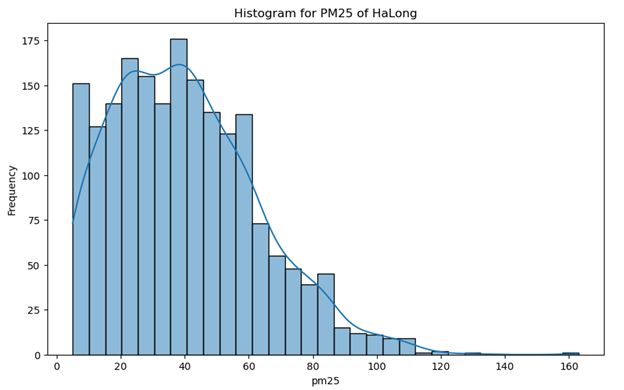
\includegraphics[width=1\textwidth]{img/final/Dataset/histogram.png}
      \end{minipage}
      \hfill
      \begin{minipage}{0.15\textwidth}
      \centering
      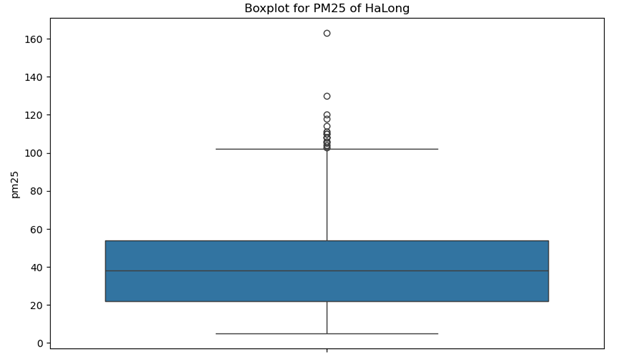
\includegraphics[width=1\textwidth]{img/final/Dataset/boxplot.png}
      \end{minipage}
      \hfill
      \begin{minipage}{0.15\textwidth}
      \centering
      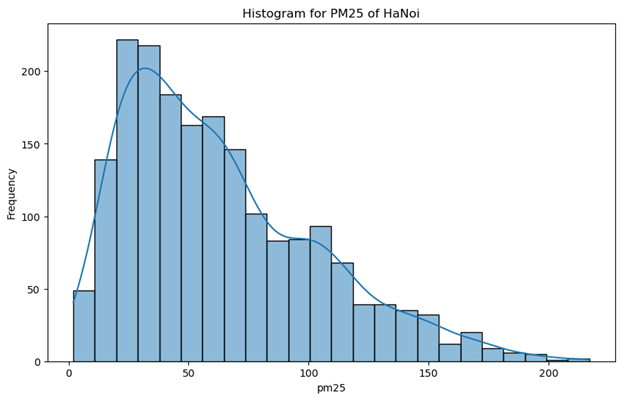
\includegraphics[width=1\textwidth]{img/final/Dataset/histogram_hn.png}
      \end{minipage}
      \hfill

  \begin{minipage}{0.15\textwidth}
      \centering
      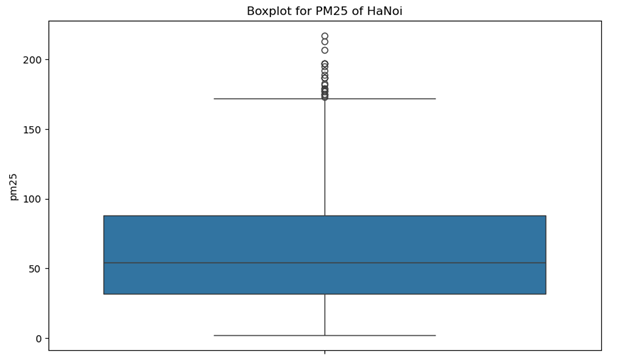
\includegraphics[width=1\textwidth]{img/final/Dataset/boxplot_hn.png}
      \end{minipage}
      \hfill
      \begin{minipage}{0.15\textwidth}
      \centering
      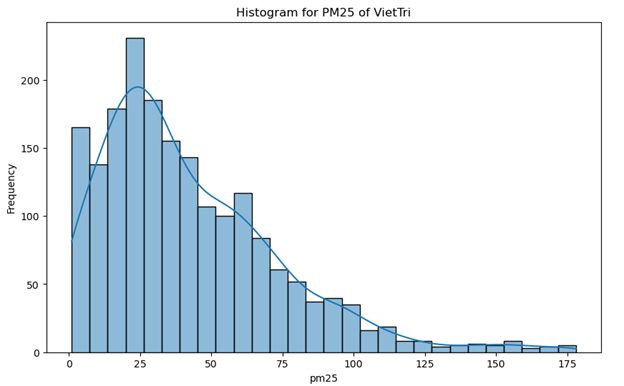
\includegraphics[width=1\textwidth]{img/final/Dataset/histogram_vt.png}
      \end{minipage}
      \hfill
      \begin{minipage}{0.15\textwidth}
      \centering
      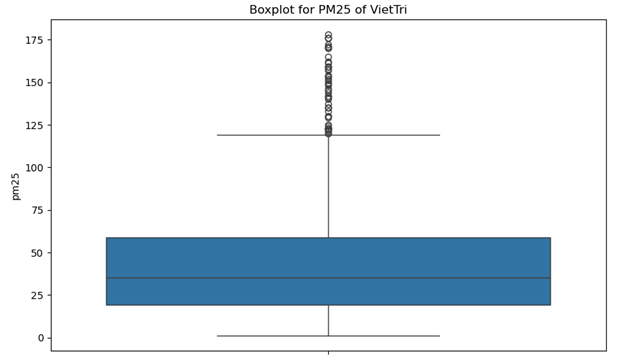
\includegraphics[width=1\textwidth]{img/final/Dataset/boxplot_vt.png}
      
      \end{minipage}
      \hfill
  
  \caption{Biểu đồ histogram và boxplot}
  \label{fig:Random_Forest}
\end{figure}

Dựa vào bảng thống kê mô tả cho Hạ Long, Hà Nội và Việt Trì, chúng ta có thể rút ra các nhận xét sau:

\textbf{Trung bình:} Hà Nội có giá trị trung bình cao nhất (63.09), tiếp theo là Việt Trì (42.39) và Hạ Long (40.08).

\textbf{Độ lệch chuẩn:} Hà Nội có độ lệch chuẩn cao nhất (40.26), cho thấy mức độ biến động lớn hơn so với Hạ Long (22.95) và Việt Trì (31.66).

\textbf{Phân vị:} Các giá trị phân vị (Q1, Q2, Q3) của Hà Nội đều cao hơn so với Hạ Long và Việt Trì, phản ánh sự phân phối dữ liệu cao hơn.

\textbf{Giá trị cực đại:} Hà Nội có giá trị cực đại cao nhất (217), trong khi Hạ Long và Việt Trì lần lượt là 163 và 178.

\textbf{Phương sai:} Hà Nội có phương sai lớn nhất (1620.88), tiếp theo là Việt Trì (1002.69) và Hạ Long (527.01).

\textbf{Độ nhọn và Độ lệch:} Việt Trì có độ nhọn (1.92) và độ lệch (1.24) cao nhất, cho thấy phân phối dữ liệu lệch về phía phải và có đỉnh cao hơn.

\textbf{Hệ số biến thiên (CV):} Việt Trì có hệ số biến thiên cao nhất (0.74), chỉ ra mức độ biến động dữ liệu lớn hơn so với Hà Nội (0.638) và Hạ Long (0.572).

\textbf{Tổng quan:} Hà Nội có giá trị trung bình cao nhất nhưng mức độ biến động và phân tán cũng lớn nhất, thể hiện sự đa dạng trong các giá trị đo lường. Việt Trì có sự biến động và phân tán dữ liệu khá cao, trong khi Hạ Long có dữ liệu ổn định hơn.


\subsection{Công cụ}
Trong quá trình nghiên cứu và phân tích dữ liệu, Nhóm đã tận dụng một loạt các công cụ phân tích thống kê trong Python để khám phá sâu hơn các mẫu dữ liệu và rút ra những kết luận có ý nghĩa. Các công cụ chính bao gồm: Darts, numpy, pandas, sklearn, matplotlib.pyplot,... Sử dụng các công cụ phân tích thống kê này đã giúp Nhóm em hiểu sâu hơn về dữ liệu và đưa ra dự báo. Chi tiết các kết quả có thể được tìm thấy trong bảng mô tả và biểu đồ đi kèm.

% \subsection{Tỷ lệ phân chia dữ liệu}
% Trong quá trình phân tích dữ liệu chuỗi thời gian, Nhóm em đã chia tập dữ liệu thành hai phần: tập huấn luyện và tập kiểm tra, với các tỷ lệ khác nhau như 70\% cho huấn luyện và 30\% cho kiểm tra, 80\% cho huấn luyện và 20\% cho kiểm tra, và 90\% cho huấn luyện và 10\% cho kiểm tra. Những tỷ lệ này giúp Nhóm đánh giá cách mà chúng ảnh hưởng đến hiệu suất của mô hình bằng cách xem xét sự phân phối của dữ liệu trong mỗi tập. Tỷ lệ phổ biến nhất là 7:3, chia 70\% dữ liệu cho huấn luyện và 30\% cho kiểm tra, tạo ra sự cân bằng giữa việc cung cấp đủ dữ liệu huấn luyện và đảm bảo các tập riêng biệt để điều chỉnh và đánh giá. Một lựa chọn khác là tỷ lệ 8:2, ưa chuộng việc sử dụng 80\% dữ liệu cho huấn luyện, có ích cho các mô hình phức tạp yêu cầu tập dữ liệu huấn luyện lớn hơn. Trong một số trường hợp cụ thể, một cách tiếp cận thận trọng như tỷ lệ 9:1 có thể được ưa chuộng, đặc biệt khi xử lý tập dữ liệu lớn và một mô hình đơn giản. Tỷ lệ này đảm bảo có đủ dữ liệu huấn luyện trong khi vẫn giữ được một tập kiểm tra đáng kể để đánh giá hiệu suất. 
\subsection{Tỷ lệ phân chia dữ liệu}
Trong quá trình phân tích dữ liệu chuỗi thời gian, Nhóm đã chia tập dữ liệu thành hai phần: tập huấn luyện và tập kiểm tra, với các tỷ lệ khác nhau như 70\% cho huấn luyện và 30\% cho kiểm tra, 80\% cho huấn luyện và 20\% cho kiểm tra, và 90\% cho huấn luyện và 10\% cho kiểm tra. Tỷ lệ phổ biến nhất là 7:3, tạo sự cân bằng giữa việc cung cấp đủ dữ liệu huấn luyện và đảm bảo các tập riêng biệt để điều chỉnh và đánh giá. Tỷ lệ 8:2 phù hợp cho các mô hình phức tạp cần nhiều dữ liệu huấn luyện, trong khi tỷ lệ 9:1 được ưa chuộng khi xử lý tập dữ liệu lớn và mô hình đơn giản.

\subsection{Đánh giá mô hình}
Trong việc đánh giá hiệu suất của các mô hình, Nhóm em sử dụng ba chỉ số là Mean Absolute Error (MAE), Mean Absolute Percentage Error (MAPE), và Root Mean Squared Error (RMSE). Thuật toán có giá trị thấp nhất trong ba chỉ số này sẽ cho thấy mức độ chính xác tốt nhất. Dưới đây là các công thức để tính MAE, MAPE và RMSE.
\subsection*{Với các tham số: }
\begin{itemize}
    \item \( n \): Số lượng điểm dữ liệu.
    \item \( y_i \): Giá trị thực tế.
    \item \( \hat{y}_i \): Giá trị dự đoán.
\end{itemize}

\subsection*{MAE (Lỗi tuyệt đối trung bình):}
MAE là trung bình của các giá trị tuyệt đối của sai số giữa giá trị dự đoán và giá trị thực tế. Nó đo lường độ lớn của sai số trung bình và không quan tâm đến hướng của sai số. MAE càng nhỏ, mô hình càng chính xác.
\begin{equation}
\text{MAE} = \frac{1}{n} \sum_{i=1}^{n} \left| y_i - \hat{y}_i \right|
\end{equation}

\subsection*{RMSE (Căn bậc hai của trung bình bình phương sai số):}
RMSE là căn bậc hai của trung bình của các bình phương của sai số giữa giá trị dự đoán và giá trị thực tế. Nó đo lường độ lớn của sai số trung bình và cung cấp một con số tương đối về mức độ sai lệch giữa dự đoán và giá trị thực tế. RMSE càng nhỏ, mô hình càng chính xác.
\begin{equation}
\text{RMSE} = \sqrt{\frac{1}{n} \sum_{i=1}^{n} (y_i - \hat{y}_i)^2}
\end{equation}

\subsection*{MAPE (Lỗi phần trăm tuyệt đối trung bình):}
MAPE là trung bình của tỉ lệ phần trăm của sai số tuyệt đối so với giá trị thực tế. Nó thường được sử dụng để đo lường tỷ lệ phần trăm trung bình của sai số so với giá trị thực tế, cung cấp cái nhìn về mức độ chính xác của mô hình dự đoán. MAPE càng nhỏ, mô hình càng chính xác.
\begin{equation}
\text{MAPE} = \frac{1}{n} \sum_{i=1}^{n} \left| \frac{y_i - \hat{y}_i}{y_i} \right| \times 100
\end{equation}
\section{Phương pháp}
\subsection{LINEAR REGRESSION}
Hồi quy tuyến tính là một kỹ thuật quan trọng trong thống kê, cho phép chúng ta khám phá và mô hình hóa mối quan hệ giữa các biến. Giúp chúng ta hiểu rõ hơn về cách các yếu tố độc lập ảnh hưởng đến một biến phụ thuộc. Trong hồi quy tuyến tính đa biến, chúng ta có thể xem xét tác động của nhiều biến độc lập đến một biến phụ thuộc, giúp tạo ra các dự đoán hoặc giải thích phức tạp hơn về thực tế. Một mô hình hồi quy tuyến tính đa biến có dạng:

\[ Y = \beta_0 + \beta_1 X_1 + \beta_2 X_2 + \ldots + \beta_k X_k + \epsilon \]

Trong đó:
\begin{itemize}
  \item \( Y \): Biến phụ thuộc.
  \item \( X_1, X_2, \ldots , X_k \): Các biến độc lập.
  \item \( \beta_0 \): Hệ số chặn
  \item \( \beta_1, \beta_2, \ldots, \beta_k \): Các hệ số hồi quy.
  \item \( \epsilon \): Thành phần sai số.
\end{itemize}
\subsection{ARIMA}

Phương pháp ARIMA (Autoregressive Integrated Moving Average) sử dụng một mô hình AR (Autoregressive) kết hợp với một mô hình MA (Moving Average) để thực hiện dự báo chuỗi thời gian. Các tham số chính cần xem xét bao gồm:

\begin{itemize}
  \item Số lượng quan sát trước đó (p);
  \item Độ chênh lệch (d);
  \item Kích thước của trung bình chuyển động (q).
\end{itemize}

Mô hình AR hiển thị sự phụ thuộc của một quan sát vào một giai đoạn thời gian trước đó. Mô hình AR thu được p quan sát trước đó như sau:

\[
y_t = \alpha + \sum_{i=1}^{p} \phi_i y_{t-i} + e_t \quad
\]

trong đó \(y_t\) là biến dự đoán cho thời điểm t từ phân phối chuẩn và \(y_{t-i}\) xác định p quan sát trước của cùng một chuỗi thời gian. \(\phi_i\) biểu thị các hệ số hồi quy, \(\alpha\) là một hằng số và \(e_t\) là thuật ngữ lỗi ngẫu nhiên. Thứ tự p cho mô hình AR(p) được lựa chọn dựa trên các đỉnh quan trọng của PACF (Partial Autocorrelation Function). Một chỉ báo bổ sung là sự giảm chậm chạp của ACF (Autocorrelation Function).

MA thực hiện dự báo dựa trên các trung bình chuyển động của các thuật ngữ lỗi ngẫu nhiên trước đó như sau:

\[
y_t = \mu + \sum_{i=1}^{q} \theta_i e_{t-i}
\]

trong đó \(\theta_t\) đại diện cho các hệ số hồi quy, q là thứ tự của trung bình chuyển động, và \(\mu\) là một hằng số. Thứ tự q cho mô hình MA(q) được lấy từ ACF, nếu nó có một đoạn cắt sắc sau lags q. PACF giảm chậm trong trường hợp này.

Mô hình ARIMA có thể được xác định như sau:

\[
\phi_p(B)(1 - B)^d y_t = \theta_q(B) e_t \quad 
\]

trong đó B là toán tử backshift, p là thứ tự tự hồi quy, d là thứ tự chênh lệch và q là thứ tự của trung bình chuyển động.
\subsection{VAR}
Mô hình Vector Autoregression (VAR) là một mô hình thống kê dùng trong phân tích chuỗi thời gian để nắm bắt mối quan hệ động giữa nhiều biến số chuỗi thời gian. Đây là sự mở rộng tự nhiên của mô hình autoregressive đơn biến sang chuỗi thời gian đa biến động. Mô hình VAR có tính linh hoạt cao trong dự báo, cho phép dự báo dựa trên các biến số cụ thể trong mô hình.

Giả sử $\mathbf{Y}_t=(y_{1t},y_{2t},\ldots,y_{nt})'$ biểu thị một vector kích thước $(n \times 1)$ chứa các biến chuỗi thời gian tại thời điểm $t$. Mô hình Vector Autoregression bậc $p$ cơ bản VAR($p$) có dạng như sau:
\[
\mathbf{Y}_t = c + \mathbf{\Pi}_1 \mathbf{Y}_{t-1} + \mathbf{\Pi}_2 \mathbf{Y}_{t-2} + \ldots + \mathbf{\Pi}_p \mathbf{Y}_{t-p} + \mathbf{\epsilon}_t, \quad t=1,\ldots,T
\]
Trong đó:
\begin{itemize}
    \item $\mathbf{Y}_t$: vector của các biến nội sinh tại thời điểm $t$, kích thước $(n \times 1)$. 
    \item $\mathbf{\Pi}_i$: các ma trận hệ số kích thước $(n \times n)$.
    \item $\mathbf{Y}_{t-1}, \mathbf{Y}_{t-2}, \ldots, \mathbf{Y}_{t-p}$: các giá trị trễ của biến nội sinh.
    \item $p$: độ trễ biểu thị các giá trị trước đó của các biến nội sinh.
    \item $\mathbf{\epsilon}_t$: vector kích thước $(n \times 1)$ của các thành phần sai số, được giả định là nhiễu trắng.
\end{itemize}

Ví dụ:
\begin{itemize}
    \item Giả sử có 2 biến nội sinh là pm25 và pm10 thì $\mathbf{Y}_t = (\text{pm25}, \text{pm10})'$. 
    \[
    \mathbf{Y}_t = \begin{pmatrix}
    \text{pm25}_t \\
    \text{pm10}_t \\
    \end{pmatrix}
    \]
    \item Ma trận chứa các hệ số cho các biến trễ của các biến nội sinh:
    \[
    \mathbf{\Pi}_1 = \begin{pmatrix}
    0.5 & 0.1 \\
    0.2 & 0.3 \\
    \end{pmatrix}
    \]
    \item Với độ trễ $p=1$, phương trình VAR(1) có dạng:
    \[
    \begin{pmatrix}
    \text{pm25}_t \\
    \text{pm10}_t \\
    \end{pmatrix} = c + \begin{pmatrix}
    0.5 & 0.1 \\
    0.2 & 0.3 \\
    \end{pmatrix} \begin{pmatrix}
    \text{pm25}_{t-1} \\
    \text{pm10}_{t-1} \\
    \end{pmatrix} + \mathbf{\epsilon}_t
    \]
\end{itemize}
\subsection{Random Forest}

\textbf{Định nghĩa}

Random Forest là phương pháp xây dựng một tập hợp cây quyết định cho các bài toán phân lớp và hồi quy. Cây quyết định thường có độ lệch thấp và phương sai cao, và Random Forest cải thiện hiệu suất bằng cách lấy trung bình các cây.

Giả sử \((X_t, Y_t)_{t \in \mathbb{Z}}\) là một dãy các biến ngẫu nhiên, trong đó:
\[ Y_t = f(X_t) + \epsilon_t \]
với \( \mathbb{E}[\epsilon_t \mid X_t] = 0 \). Mục tiêu là ước lượng hàm hồi quy 
\[ f(x) = \mathbb{E}[Y_t \mid X_t = x] \]
\textbf{Block Bootstrap cho Chuỗi Thời Gian:}
\begin{itemize}
    \item \textbf{Moving Block Bootstrap:} Chia dữ liệu thành các khối chồng lấn kích thước cố định, lấy mẫu lại để tạo chuỗi mới.
    \item \textbf{Circular Block Bootstrap:} Bao bọc chuỗi thời gian theo vòng tròn, đảm bảo điểm dữ liệu đều đại diện.
\end{itemize}
\textbf{Thuật Toán:}
\begin{itemize}
    \item \textbf{Đầu Vào:} Dữ liệu huấn luyện \( \{ (X_1, Y_1), \ldots, (X_n, Y_n) \} \), các tham số \( M, \alpha_n, m_{try}, \tau_n, l_n \).
    \item \textbf{Xây Dựng Cây cho \( j = 1 \) đến \( M \):}
    \begin{itemize}
        \item Lấy \( \alpha_n \) quan sát bằng block bootstrap với tham số \( l_n \).
        \item Chia nút chọn chia cắt tốt nhất từ tập con ngẫu nhiên của \( m_{try} \) đặc trưng.
    \end{itemize}
    \item \textbf{Đầu Ra:} Dự đoán cho một quan sát mới \( x \) là trung bình của dự đoán từ \( M \) cây:
    \[ \hat{f}(x) = \frac{1}{M} \sum_{j=1}^{M} \hat{f}_j(x) \]
\end{itemize}

\subsection{Time-series Dense Encoder}
\textbf{TiDE} (Time-series Dense Encoder) là một mô hình dự báo chuỗi thời gian. Mô hình mã hóa chuỗi thời gian quá khứ cùng với hiệp phương sai bằng cách sử dụng “dense MLP” (Multi-Layer Perceptron). Sau đó, mô hình giải mã (decode) chuỗi thời gian được mã hóa (encode) cùng với các hiệp phương sai trong tương lai.
\begin{figure}[h]
    \centering
    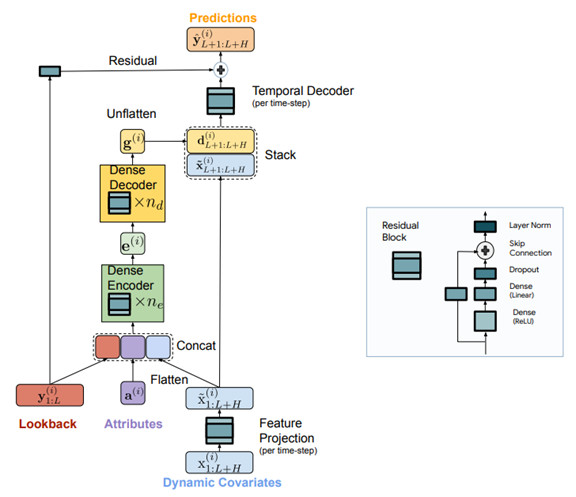
\includegraphics[width=0.5\textwidth]{img/TiDE.png}
    \caption{Tổng quan về kiến trúc TiDE}
    \label{fig:your_figure_label}
\end{figure}

\text{Kiến trúc tổng quan được trình bày ở Hình 4.} Đầu vào (input) của mô hình là dữ liệu quá khứ và phương sai của một chuỗi thời gian tại một thời điểm ($y_{1:L}^{(i)}, x_{1:L}^{(i)}, a^{(i)}$) và ánh xạ tới dự đoán của chuỗi thời gian $\hat{y}_{L+1:L+H}^{(i)}$.

\textbf{Residual Block:} Là một thành phần quan trọng của kiến trúc TiDE vì nó cho phép mô hình nắm bắt các tính chất phi tuyến tính vốn có trong dữ liệu chuỗi thời gian, đồng thời duy trì các mối quan hệ tuyến tính nhằm giúp cải thiện hiệu suất dự báo dài hạn. 

Giả sử đầu vào của Residual Block là \( \mathbf{x} \), công thức của nó có thể được mô tả như sau:

\begin{itemize}
    \item Layer Normalization:
    \[
    \mathbf{h}_0 = \text{LayerNorm}(\mathbf{x})
    \]

    \item Lớp Dense đầu tiên với ReLU Activation:
    \[
    \mathbf{h}_1 = \text{ReLU}(\mathbf{W}_1 \mathbf{h}_0 + \mathbf{b}_1)
    \]

    \item Dropout (tùy chọn):
    \[
    \mathbf{h}_1 = \text{Dropout}(\mathbf{h}_1, p)
    \]
    Trong đó, \( p \) là xác suất giữ lại của Dropout.

    \item Lớp Dense thứ hai:
    \[
    \mathbf{h}_2 = \mathbf{W}_2 \mathbf{h}_1 + \mathbf{b}_2
    \]

    \item  ReLU Activation sau Kết nối tắt (Skip Connection):
    \[
    \tilde{\mathbf{x}} = \text{ReLU}(\mathbf{x} + \mathbf{h}_2)
    \]

\end{itemize}

Trong đó:
\begin{itemize}
    \item \( \mathbf{W}_1 \) và \( \mathbf{W}_2 \) là các ma trận trọng số của các lớp Dense MLP.
    \item \( \mathbf{b}_1 \) và \( \mathbf{b}_2 \) là các vector bù.
    \item \(\text{LayerNorm}(\cdot)\) là hàm chuẩn hóa lớp.
    \item \(\text{Dropout}(\cdot, p)\) là hàm Dropout với xác suất \( p \).
    \item \(\text{ReLU}(\cdot)\) là hàm kích hoạt ReLU.
    \item \(\tilde{\mathbf{x}}\) là đầu ra của Residual Block.
\end{itemize}

\textbf{Mã hóa (Encoding):}
\begin{itemize}
    \item \textbf{Feature Projection:} Sử dụng residual block để ánh xạ \( x_t^{(i)} \) tại mỗi time-step, hoạt động này được mô tả như sau:
    \[
        \tilde{x}_t^{(i)} = \text{ResidualBlock}(x_t^{(i)}) 
    \]

    \item \textbf{Dense Encoder:} Xếp chồng và làm phẳng tất cả các biến động trong quá khứ và tương lai, nối chúng với các thuộc tính tĩnh và quá khứ của chuỗi thời gian. Ánh xạ vào một embedding bằng cách sử dụng một bộ mã hóa chứa nhiều khối dư:
    \[
    e^{(i)} = \text{Encoder}\left( y_{1:L}^{(i)}, \tilde{x}_{1:L}^{(i)}, \tilde{x}_{1:L+H}^{(i)}, a^{(i)} \right)
    \]
\end{itemize}

\textbf{Giải mã (Decoding):}

\begin{itemize}
    \item \textbf{Dense Decoder (Bộ giải mã dense):} Đơn vị giải mã đầu tiên xếp chồng nhiều khối dư giống bộ mã hóa với cùng kích thước lớp ẩn, nhận đầu vào là mã hóa \( e^{(i)} \), ánh xạ thành vector \( g^{(i)} \) kích thước \( H \times p \) (\texttt{decoderOutputDim}), và chuyển đổi thành ma trận \( D^{(i)} \in \mathbb{R}^{p \times H} \):
    \[
    g^{(i)} = \text{Decoder}(e^{(i)}) \in \mathbb{R}^{p \times H}
    \]
    \[
    D^{(i)} = \text{Reshape}(g^{(i)}) \in \mathbb{R}^{p \times H}
    \]

    \item \textbf{Temporal Decoder (Bộ giải mã thời gian):} Cuối cùng, bộ giải mã thời gian, một khối dư với đầu ra kích thước 1, ánh xạ vector \( d^{(i)}_t \) tại thời điểm \( t \) kết hợp với các phương sai đã được chiếu \( \tilde{x}^{(i)}_{L+t} \):
    \[
    \hat{y}^{(i)}_{L+t} = \text{TemporalDecoder}(d^{(i)}_t, \tilde{x}^{(i)}_{L+t}) \quad \forall t \in [H]
    \]
\end{itemize}
\subsection{RNN}
Mạng nơ-ron hồi tiếp (RNN) là một loại mạng có khả năng xử lý dữ liệu tuần tự. Điểm đặc biệt của RNN là các nơ-ron trong mạng có thể kết nối với nhau theo chu kỳ. Nhờ vậy, RNN có thể học được mối quan hệ giữa các giá trị trong một chuỗi thời gian.

Công thức biểu diễn của RNN như sau:
\begin{equation}
h_t = f(x_t, h_{t-1})
\end{equation}
Trong đó:
\begin{itemize}
    \item $h_t$: trạng thái của RNN tại thời điểm $t$
    \item $x_t$: đầu vào của RNN tại thời điểm $t$
    \item $h_{t-1}$: trạng thái của RNN tại thời điểm $t - 1$
    \item $f$: hàm kích hoạt của RNN
\end{itemize}
\documentclass{article}
\usepackage{amsmath}
\usepackage{amsfonts}
\usepackage{graphicx}
\usepackage{hyperref}


\begin{document}

\section{Giới thiệu và Khái niệm}

Trong lĩnh vực học máy và đặc biệt là xử lý ngôn ngữ tự nhiên (NLP), mạng nơ-ron hồi tiếp (Recurrent Neural Networks - RNNs) đóng vai trò quan trọng. Tuy nhiên, RNN truyền thống gặp phải vấn đề về vanishing gradient, làm giảm hiệu quả học của mạng khi xử lý các chuỗi dữ liệu dài. Để giải quyết vấn đề này, các kiến trúc RNN cải tiến như Long Short-Term Memory (LSTM) và Gated Recurrent Unit (GRU) đã được đề xuất. Bài viết này tập trung vào Gated Recurrent Unit (GRU), một biến thể đơn giản hơn của LSTM nhưng vẫn rất hiệu quả trong việc duy trì thông tin dài hạn.

GRU được giới thiệu bởi Kyunghyun Cho et al. vào năm 2014. Điểm nổi bật của GRU là sự kết hợp giữa các cơ chế cập nhật và quên trong một đơn vị duy nhất, giúp giảm thiểu số lượng tham số cần thiết và tăng tốc độ tính toán mà vẫn duy trì hiệu quả cao.

\section{Mô tả Chi tiết Thuật toán}

Một GRU bao gồm hai cổng chính: cổng cập nhật (update gate) và cổng xoá (reset gate). Cả hai cổng này cùng hoạt động để điều chỉnh thông tin nào cần được cập nhật và thông tin nào cần được quên. 

\subsection{Công thức Toán học}

Cho \( x_t \) là đầu vào tại thời điểm \( t \), \( h_t \) là trạng thái ẩn tại thời điểm \( t \), và \( h_{t-1} \) là trạng thái ẩn từ bước trước đó, các công thức của GRU được định nghĩa như sau:

\subsubsection{Cổng Cập Nhật}

Cổng cập nhật \( z_t \) quyết định phần nào của trạng thái ẩn trước đó cần được giữ lại và phần nào cần được cập nhật:

\[
z_t = \sigma(W_z x_t + U_z h_{t-1})
\]

\subsubsection{Cổng Xoá}

Cổng xoá \( r_t \) quyết định phần nào của trạng thái ẩn trước đó cần được quên:

\[
r_t = \sigma(W_r x_t + U_r h_{t-1})
\]

\subsubsection{Trạng Thái Ẩn Mới}

Trạng thái ẩn mới \( \tilde{h}_t \) được tính toán bằng cách sử dụng cổng xoá để điều chỉnh thông tin từ trạng thái ẩn trước đó:

\[
\tilde{h}_t = \tanh(W_h x_t + U_h (r_t \odot h_{t-1}))
\]

\subsubsection{Cập Nhật Trạng Thái Ẩn Cuối Cùng}

Trạng thái ẩn cuối cùng \( h_t \) tại thời điểm \( t \) được tính bằng cách kết hợp trạng thái ẩn trước đó và trạng thái ẩn mới theo trọng số của cổng cập nhật:

\[
h_t = (1 - z_t) \odot h_{t-1} + z_t \odot \tilde{h}_t
\]

\subsection{Diễn Giải Các Cổng}

\begin{itemize}
    \item \textbf{Cổng cập nhật} \( z_t \): Quyết định tỉ lệ mà trạng thái ẩn trước đó được giữ lại so với trạng thái ẩn mới.
    \item \textbf{Cổng xoá} \( r_t \): Điều chỉnh thông tin nào của trạng thái ẩn trước đó được sử dụng để tính toán trạng thái ẩn mới.
\end{itemize}

\subsection{Ưu Điểm của GRU}

GRU có một số ưu điểm so với các kiến trúc RNN truyền thống và cả LSTM:

\begin{itemize}
    \item \textbf{Đơn giản hóa} nhờ ít tham số hơn so với LSTM, giúp giảm thiểu chi phí tính toán.
    \item \textbf{Hiệu quả} trong việc xử lý các chuỗi dài mà không gặp phải vấn đề vanishing gradient nghiêm trọng.
    \item \textbf{Tốc độ huấn luyện} nhanh hơn do kiến trúc gọn nhẹ hơn.
\end{itemize}

\begin{thebibliography}{9}
\bibitem{cho2014} Kyunghyun Cho, Bart van Merriënboer, Dzmitry Bahdanau, Yoshua Bengio. \textit{On the Properties of Neural Machine Translation: Encoder-Decoder Approaches}. 2014.
\end{thebibliography}

\end{document}

\subsection{LSTM}

LSTM là một loại mạng nơ-ron tái hiện (RNN) được thiết kế để xử lý và dự báo chuỗi thời gian. Nó khắc phục các vấn đề về Vanishing Gradient (Đạo hàm bị triệt tiêu) và Exploding Gradient (Bùng nổ đạo hàm) trong các RNN truyền thống, cho phép mô hình lưu trữ thông tin trong thời gian dài. LSTM gồm các đơn vị nhớ (memory cell) với ba cổng chính: cổng quên (forget gate), cổng đầu vào (input gate), và cổng đầu ra (output gate). Các cổng này điều khiển dòng thông tin qua đơn vị nhớ.

\paragraph{Cổng Quên (Forget Gate)}
Cổng quên quyết định lượng thông tin từ trạng thái trước đó cần được giữ lại hoặc loại bỏ:
\[
f_t = \sigma(W_f \cdot [h_{t-1}, x_t] + b_f)
\]
trong đó, \(f_t\) là giá trị của cổng quên tại thời điểm \(t\), \(W_f\) là trọng số của cổng quên, \(h_{t-1}\) là đầu ra từ bước thời gian trước, \(x_t\) là đầu vào tại thời điểm \(t\), và \(b_f\) là giá trị bias của cổng quên.

\paragraph{Cổng Đầu Vào (Input Gate)}
Cổng đầu vào xác định lượng thông tin mới cần được lưu trữ trong trạng thái nhớ:
\[
i_t = \sigma(W_i \cdot [h_{t-1}, x_t] + b_i)
\]
\[
\tilde{C}_t = \tanh(W_C \cdot [h_{t-1}, x_t] + b_C)
\]
trong đó, \(i_t\) là giá trị của cổng đầu vào, \(W_i\) là trọng số của cổng đầu vào, \(\tilde{C}_t\) là giá trị của thông tin mới, \(W_C\) là trọng số của thông tin mới, và \(b_i\), \(b_C\) lần lượt là các giá trị bias của cổng đầu vào và thông tin mới.

\paragraph{Cập Nhật Trạng Thái Nhớ}
Trạng thái nhớ được cập nhật bằng cách kết hợp trạng thái cũ và thông tin mới:
\[
C_t = f_t \cdot C_{t-1} + i_t \cdot \tilde{C}_t
\]
trong đó, \(C_t\) là trạng thái nhớ tại thời điểm \(t\) và \(C_{t-1}\) là trạng thái nhớ từ bước thời gian trước.

\paragraph{Cổng Đầu Ra (Output Gate)}
Cổng đầu ra xác định đầu ra của đơn vị LSTM dựa trên trạng thái nhớ hiện tại:
\[
o_t = \sigma(W_o \cdot [h_{t-1}, x_t] + b_o)
\]
\[
h_t = o_t \cdot \tanh(C_t)
\]
trong đó, \(o_t\) là giá trị của cổng đầu ra, \(W_o\) là trọng số của cổng đầu ra, \(b_o\) là giá trị bias của cổng đầu ra, và \(h_t\) là đầu ra của đơn vị LSTM tại thời điểm \(t\).

Các cổng trong LSTM kiểm soát dòng thông tin qua các đơn vị nhớ, giúp mô hình duy trì và cập nhật trạng thái nhớ một cách hiệu quả và chính xác. Điều này giải quyết các vấn đề đạo hàm bị triệt tiêu và bùng nổ đạo hàm, cải thiện hiệu quả dự đoán cho các bài toán chuỗi thời gian.
\documentclass[a4paper, 12pt]{article}
\usepackage[utf8]{inputenc}
\usepackage{amsmath}
\usepackage{amsfonts}
\usepackage{amssymb}
\usepackage{graphicx}
\usepackage{hyperref}

\title{Multi-Layer Perceptron}
\date{\today}

\begin{document}

\section{Giới thiệu và Khái Niệm}

Multi-Layer Perceptron (MLP) là một loại mạng nơ-ron nhân tạo, là một phần của học sâu (deep learning). MLP bao gồm ít nhất ba lớp: một lớp đầu vào, một hoặc nhiều lớp ẩn, và một lớp đầu ra. Mỗi lớp chứa nhiều nơ-ron (neurons), và mỗi nơ-ron trong một lớp kết nối với tất cả các nơ-ron trong lớp kế tiếp.

MLP có thể được sử dụng cho nhiều nhiệm vụ khác nhau như phân loại, hồi quy và dự báo chuỗi thời gian. Mỗi nơ-ron trong MLP sử dụng một hàm kích hoạt phi tuyến tính để tạo ra đầu ra của nó, giúp mạng có khả năng học các mối quan hệ phi tuyến giữa đầu vào và đầu ra.

\section{Mô Tả Chi Tiết Thuật Toán}

\subsection{Thuật Toán Gradient Descent}

Gradient descent là một phương pháp tối ưu hóa phổ biến được sử dụng để tìm cực tiểu của hàm mất mát (loss function). Trong ngữ cảnh của MLP, hàm mất mát đo lường sự khác biệt giữa dự đoán của mạng và giá trị thực tế.

Công thức cập nhật trọng số trong gradient descent như sau:
\[
\theta_{i} := \theta_{i} - \eta \frac{\partial J(\theta)}{\partial \theta_{i}}
\]
trong đó, \(\theta_{i}\) là trọng số cần cập nhật, \(\eta\) là tốc độ học (learning rate), và \(J(\theta)\) là hàm mất mát.

\subsection{Thuật Toán Backpropagation}

Backpropagation là một phương pháp hiệu quả để tính gradient của hàm mất mát đối với các trọng số của MLP. Quá trình backpropagation bao gồm hai bước chính: lan truyền tiến (forward propagation) và lan truyền ngược (backward propagation).

Trong bước lan truyền tiến, chúng ta tính toán đầu ra của mạng cho một đầu vào cụ thể. Trong bước lan truyền ngược, chúng ta tính toán gradient của hàm mất mát đối với từng trọng số bằng cách áp dụng quy tắc dây chuyền (chain rule).

\subsection{Feedforward}

Feedforward là quá trình tính toán đầu ra của mạng từ đầu vào bằng cách đi qua các lớp nơ-ron. Quá trình này bao gồm việc tính toán đầu ra của mỗi nơ-ron trong lớp ẩn và lớp đầu ra.

Giả sử \(a^{(l)}\) là đầu ra của lớp \(l\), quá trình feedforward được mô tả như sau:
\[
z^{(l+1)} = W^{(l)}a^{(l)} + b^{(l)}
\]
\[
a^{(l+1)} = \sigma(z^{(l+1)})
\]
trong đó, \(W^{(l)}\) và \(b^{(l)}\) lần lượt là trọng số và bias của lớp \(l\), \(z^{(l+1)}\) là tổng trọng số, và \(\sigma\) là hàm kích hoạt.

\section{Kết Luận}

Multi-Layer Perceptron là một mô hình cơ bản nhưng mạnh mẽ trong học sâu, có thể áp dụng vào nhiều bài toán khác nhau. Việc hiểu rõ các thuật toán gradient descent, backpropagation và feedforward là cần thiết để tối ưu hóa và huấn luyện MLP hiệu quả.

\end{document}

\subsection{Autoformer}

Autoformer là một mô hình được thiết kế để dự báo chuỗi thời gian dài hạn, bao gồm ba thành phần chính: Khối phân rã chuỗi (Series Decomposition Block), Cơ chế tự tương quan (Auto-Correlation Mechanism), và Bộ mã hóa/giải mã (Encoder/Decoder).

\subsubsection{Khối Phân Rã Chuỗi}

Khối phân rã chuỗi được sử dụng để tách chuỗi thời gian thành các thành phần xu hướng và mùa vụ. Phương pháp này sử dụng trung bình động để làm mượt các dao động định kỳ và làm nổi bật xu hướng dài hạn. Công thức cơ bản như sau:

\[
X_t = \text{AvgPool}(\text{Padding}(X))
\]
\[
X_s = X - X_t
\]

Trong đó, \(X_s\) và \(X_t\) lần lượt là các phần mùa vụ và xu hướng của chuỗi.

\subsubsection{Cơ Chế Tự Tương Quan}

Cơ chế tự tương quan được thiết kế để phát hiện các phụ thuộc dựa trên chu kỳ và tập hợp các chuỗi con tương tự từ các chu kỳ ngầm. Cơ chế này thay thế cho self-attention trong Transformer và có độ phức tạp \(O(L \log L)\), trong đó \(L\) là chiều dài chuỗi.

\paragraph{Công Thức Tự Tương Quan}

Cơ chế tự tương quan bao gồm hai bước chính: tính toán tự tương quan và tổng hợp các giá trị tương quan.

\[
\text{ACF}(X, \tau) = \frac{1}{L} \sum_{t=1}^{L-\tau} X_t \cdot X_{t+\tau}
\]

Trong đó, \(\text{ACF}(X, \tau)\) là hàm tự tương quan, \(X_t\) là giá trị tại thời điểm \(t\), và \(\tau\) là độ trễ.

Sau khi tính toán hàm tự tương quan, các giá trị được tổng hợp lại để tìm các chuỗi con tương tự, dựa trên công thức:

\[
Y_{t+\tau} = \sum_{k=1}^{K} \alpha_k X_{t+\tau_k}
\]

Trong đó, \(\alpha_k\) là trọng số tự tương quan, và \(K\) là số lượng chuỗi con được chọn.

\subsubsection{Bộ Mã Hóa và Bộ Giải Mã}

Bộ mã hóa và bộ giải mã của Autoformer bao gồm các khối phân rã chuỗi và cơ chế tự tương quan. Bộ mã hóa xử lý dữ liệu đầu vào từ chuỗi thời gian quá khứ, trong khi bộ giải mã tinh chỉnh các thành phần mùa vụ và xu hướng để đưa ra dự báo.

\paragraph{Bộ mã hóa (Encoder)}

Bộ mã hóa bao gồm các khối phân rã và cơ chế tự tương quan để xử lý và trích xuất thông tin từ chuỗi đầu vào. Định nghĩa các hàm được sử dụng như sau:

\begin{itemize}
    \item \textbf{Decompose(X)}: Hàm này phân rã chuỗi thời gian \(X\) thành các thành phần xu hướng (\(X_t\)) và mùa vụ (\(X_s\)).
    \item \textbf{AutoCorrelation(H)}: Hàm này tính toán tự tương quan của chuỗi \(H\) để tìm các chuỗi con tương tự và các phụ thuộc chu kỳ trong dữ liệu.
\end{itemize}

\[
\begin{aligned}
    H^{(l)} &= \text{Decompose}(X^{(l)}) \\
    Z^{(l)} &= \text{AutoCorrelation}(H^{(l)})
\end{aligned}
\]

    
Trong đó, \(H^{(l)}\) là đầu ra của lớp phân rã thứ \(l\), và \(Z^{(l)}\) là đầu ra của lớp tự tương quan thứ \(l\).
    
\paragraph{Bộ giải mã (Decoder)}
    
Bộ giải mã nhận các thành phần xu hướng và mùa vụ từ bộ mã hóa và tiếp tục tinh chỉnh, sử dụng các khối phân rã và cơ chế tự tương quan để dự báo chuỗi thời gian trong tương lai. Định nghĩa các hàm cũng tương tự như trong bộ mã hóa:

\[
\begin{aligned}
    \hat{Y}^{(l)} &= \text{Decompose}(Z^{(l)}) \\
    \hat{X}^{(l)} &= \text{AutoCorrelation}(\hat{Y}^{(l)})
\end{aligned}
\]
\section{Kết quả thí nghiệm}
\subsection{Cài đặt mô hình}

\begin{figure}[H]
    \makebox[\textwidth][l]{1. Linear Regression}

    \centering
    \begin{minipage}{0.15\textwidth}
    \centering
    \end{minipage}
    \hfill

    \begin{minipage}{0.15\textwidth}
        \centering
        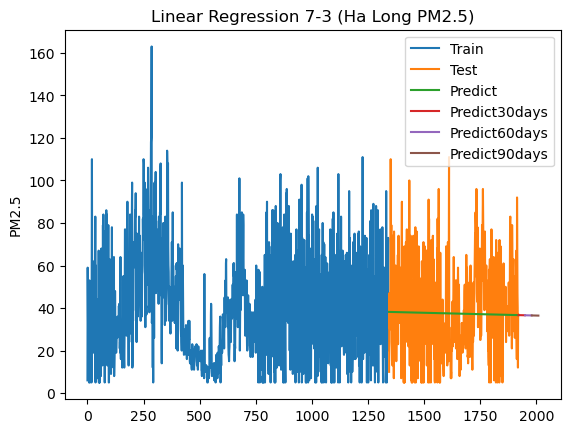
\includegraphics[width=1\textwidth]{img/final/Linear Regression/90D/LN_7_3_HL.png}
        \end{minipage}
        \hfill
        \begin{minipage}{0.15\textwidth}
        \centering
        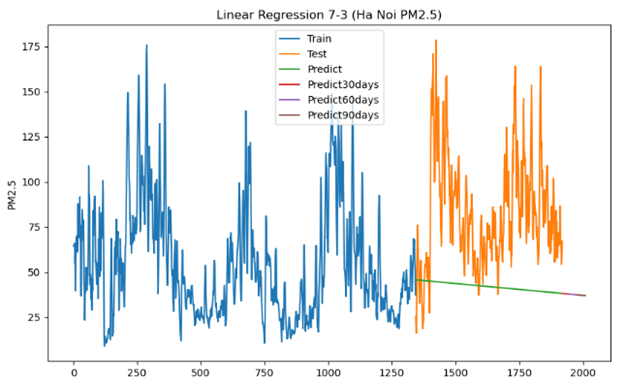
\includegraphics[width=1\textwidth]{img/final/Linear Regression/90D/LN_7_3_HN.png}
        \end{minipage}
        \hfill
        \begin{minipage}{0.15\textwidth}
        \centering
        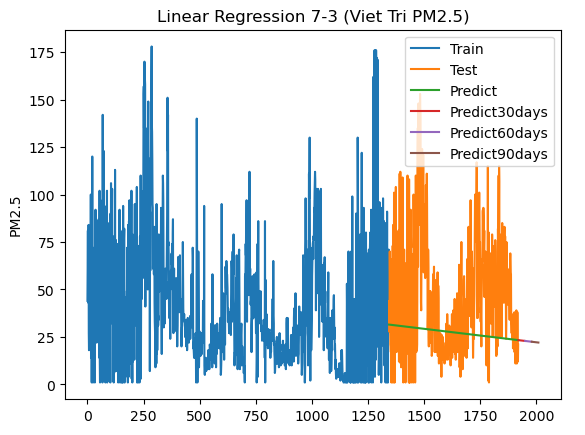
\includegraphics[width=1\textwidth]{img/final/Linear Regression/90D/LN_7_3_VT.png}
        \end{minipage}
        \hfill

    \begin{minipage}{0.15\textwidth}
        \centering
        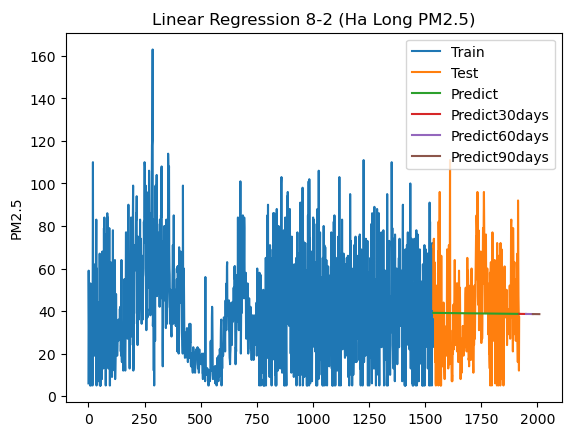
\includegraphics[width=1\textwidth]{img/final/Linear Regression/90D/LN_8_2_HL.png}
        \end{minipage}
        \hfill
        \begin{minipage}{0.15\textwidth}
        \centering
        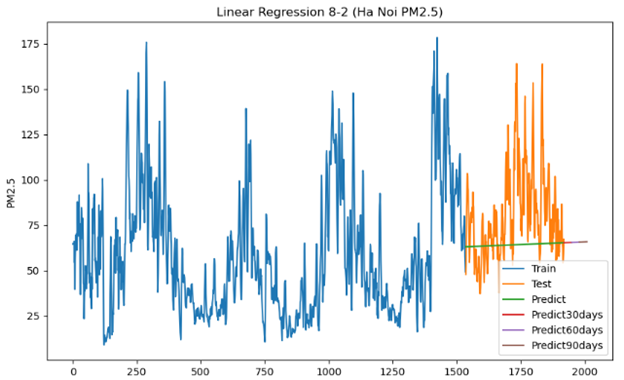
\includegraphics[width=1\textwidth]{img/final/Linear Regression/90D/LN_8_2_HN.png}
        \end{minipage}
        \hfill
        \begin{minipage}{0.15\textwidth}
        \centering
        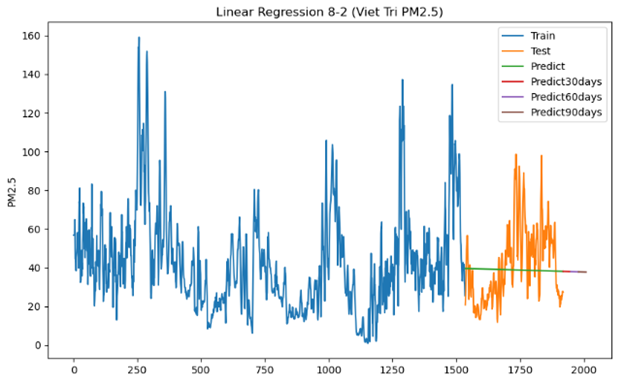
\includegraphics[width=1\textwidth]{img/final/Linear Regression/90D/LN_8_2_VT.png}
        \end{minipage}
        \hfill

    \begin{minipage}{0.15\textwidth}
        \centering
        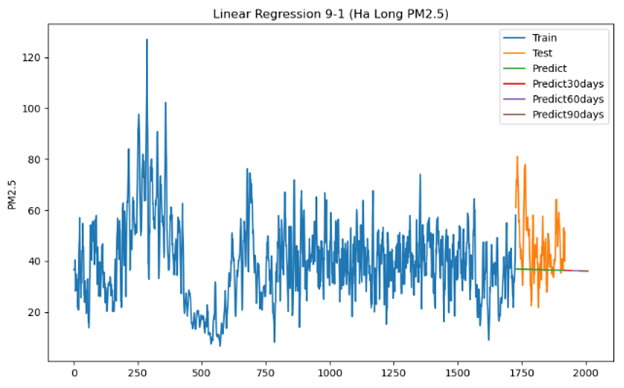
\includegraphics[width=1\textwidth]{img/final/Linear Regression/90D/LN_9_1_HL.png}
        \end{minipage}
        \hfill
        \begin{minipage}{0.15\textwidth}
        \centering
        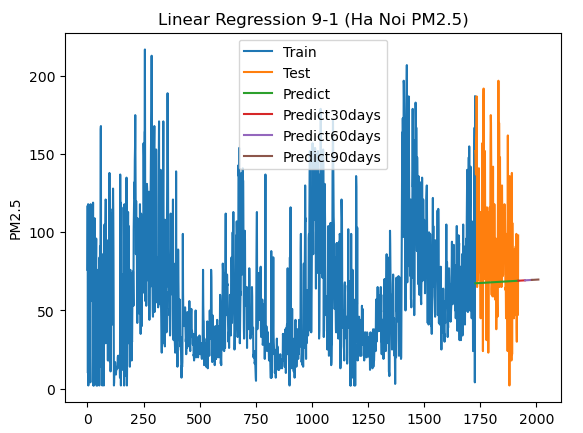
\includegraphics[width=1\textwidth]{img/final/Linear Regression/90D/LN_9_1_HN.png}
        \end{minipage}
        \hfill
        \begin{minipage}{0.15\textwidth}
        \centering
        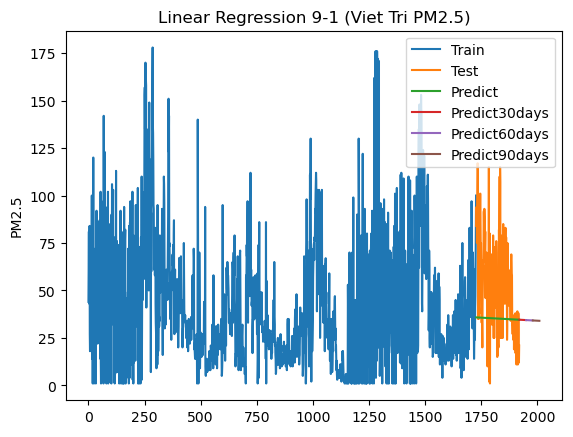
\includegraphics[width=1\textwidth]{img/final/Linear Regression/90D/LN_9_1_VT.png}
        \end{minipage}
        \hfill
    
    \caption{Kết quả dự báo của mô hình Linear Regression}
    \label{fig:LN}
    
\end{figure}


\begin{figure}[H]
    \makebox[\textwidth][l]{2. ARIMA}

    \centering
    \begin{minipage}{0.15\textwidth}
    \centering
    \end{minipage}
    \hfill

    \begin{minipage}{0.15\textwidth}
    \centering
    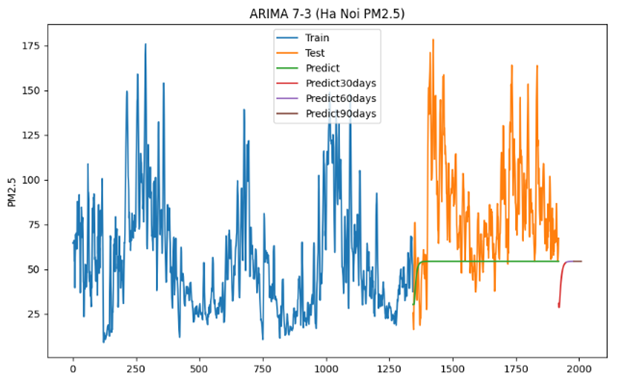
\includegraphics[width=1\textwidth]{img/final/ARIMA/90D/ARIMA_7_3_HN.png}
    \end{minipage}
    \hfill
    \begin{minipage}{0.15\textwidth}
    \centering
    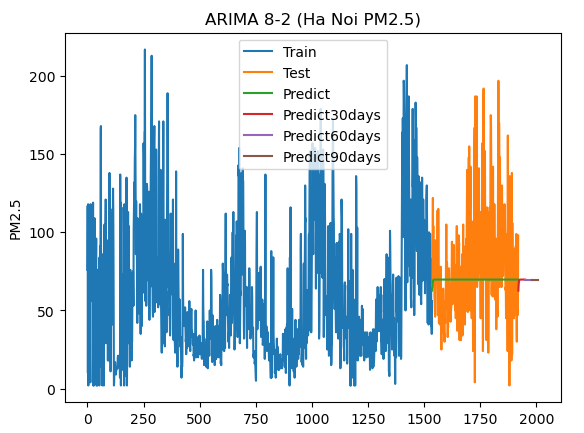
\includegraphics[width=1\textwidth]{img/final/ARIMA/90D/ARIMA_8_2_HN.png}
    \end{minipage}
    \hfill
    \begin{minipage}{0.15\textwidth}
    \centering
    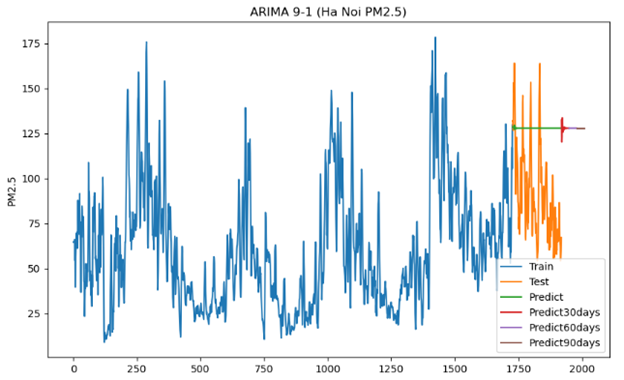
\includegraphics[width=1\textwidth]{img/final/ARIMA/90D/ARIMA_9_1_HN.png}
    \end{minipage}
    \hfill

    \begin{minipage}{0.15\textwidth}
    \centering
    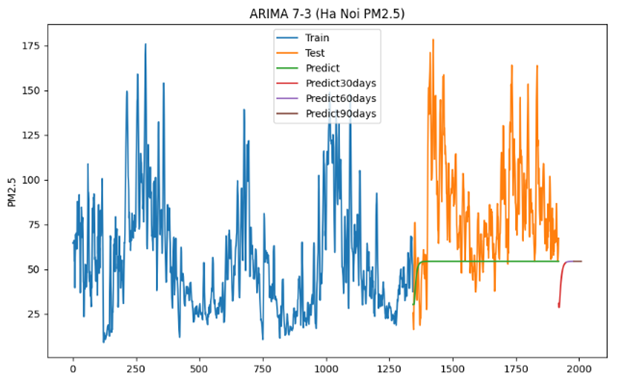
\includegraphics[width=1\textwidth]{img/final/ARIMA/90D/ARIMA_7_3_HN.png}
    \end{minipage}
    \hfill
    \begin{minipage}{0.15\textwidth}
    \centering
    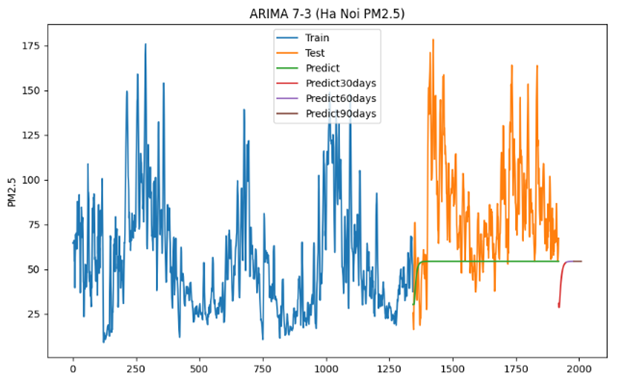
\includegraphics[width=1\textwidth]{img/final/ARIMA/90D/ARIMA_7_3_HN.png}
    \end{minipage}
    \hfill
    \begin{minipage}{0.15\textwidth}
    \centering
    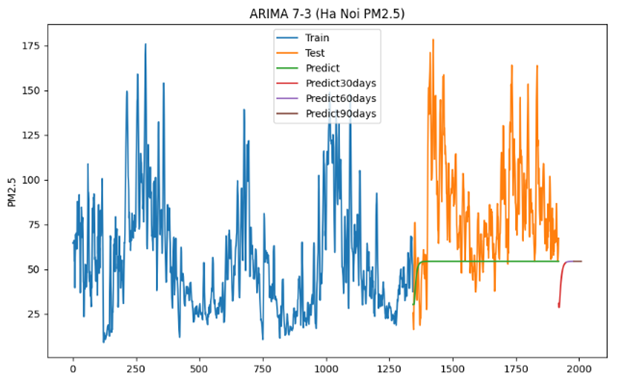
\includegraphics[width=1\textwidth]{img/final/ARIMA/90D/ARIMA_7_3_HN.png}
    \end{minipage}
    \hfill

    \begin{minipage}{0.15\textwidth}
    \centering
    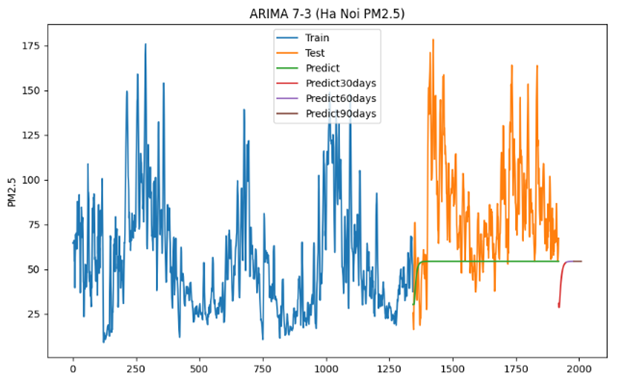
\includegraphics[width=1\textwidth]{img/final/ARIMA/90D/ARIMA_7_3_HN.png}
    \end{minipage}
    \hfill
    \begin{minipage}{0.15\textwidth}
    \centering
    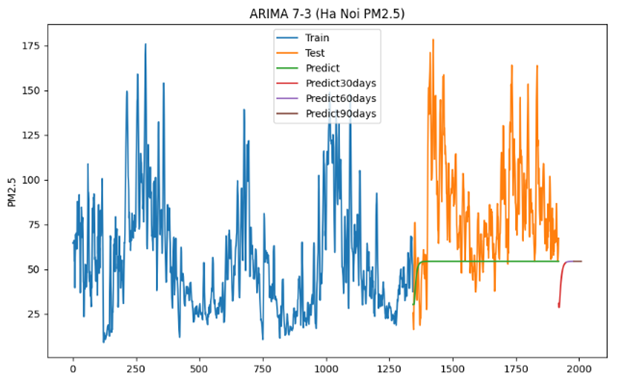
\includegraphics[width=1\textwidth]{img/final/ARIMA/90D/ARIMA_7_3_HN.png}
    \end{minipage}
    \hfill
    \begin{minipage}{0.15\textwidth}
    \centering
    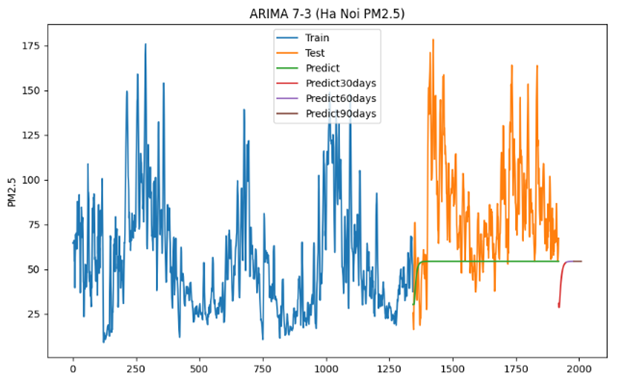
\includegraphics[width=1\textwidth]{img/final/ARIMA/90D/ARIMA_7_3_HN.png}
    \end{minipage}
    \hfill
    
    \caption{Kết quả chạy của mô hình ARIMA}
    \label{fig:ARIMA}
\end{figure}


\begin{figure}[H]
    \makebox[\textwidth][l]{2. VAR}

    \centering
    \begin{minipage}{0.15\textwidth}
    \centering
    \end{minipage}
    \hfill

    \begin{minipage}{0.15\textwidth}
    \centering
    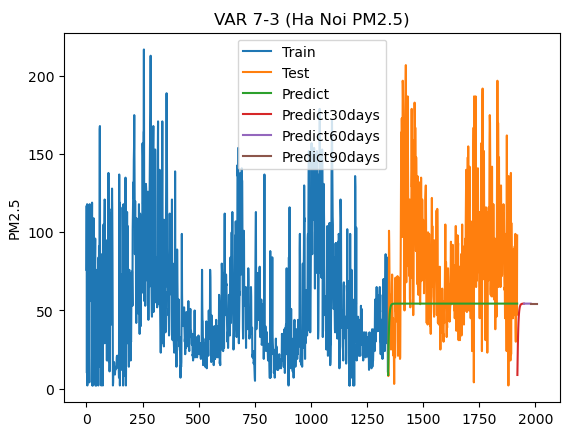
\includegraphics[width=1\textwidth]{img/final/VAR/90D/VAR_7_3_HN.png}
    \end{minipage}
    \hfill
    \begin{minipage}{0.15\textwidth}
    \centering
    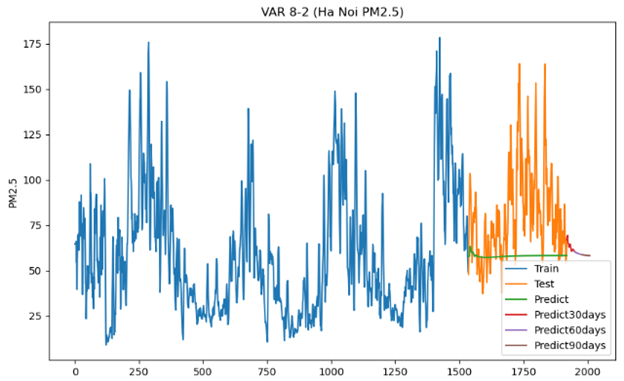
\includegraphics[width=1\textwidth]{img/final/VAR/90D/VAR_8_2_HN.png}
    \end{minipage}
    \hfill
    \begin{minipage}{0.15\textwidth}
    \centering
    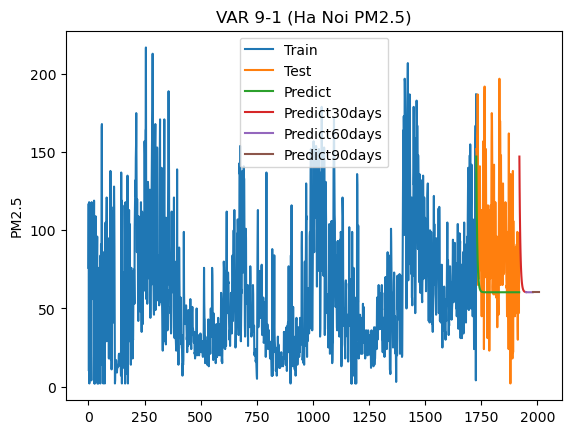
\includegraphics[width=1\textwidth]{img/final/VAR/90D/VAR_9_1_HN.png}
    \end{minipage}
    \hfill

    \begin{minipage}{0.15\textwidth}
    \centering
    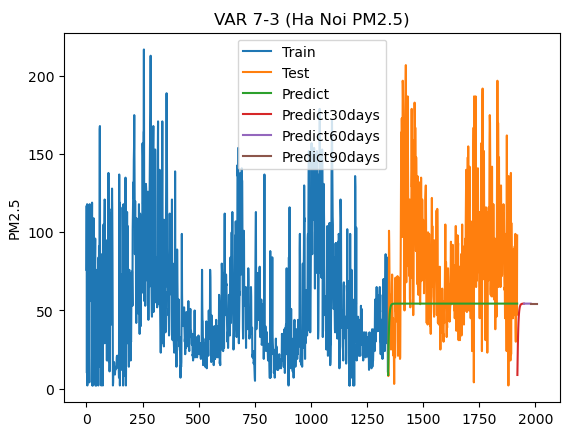
\includegraphics[width=1\textwidth]{img/final/VAR/90D/VAR_7_3_HN.png}
    \end{minipage}
    \hfill
    \begin{minipage}{0.15\textwidth}
    \centering
    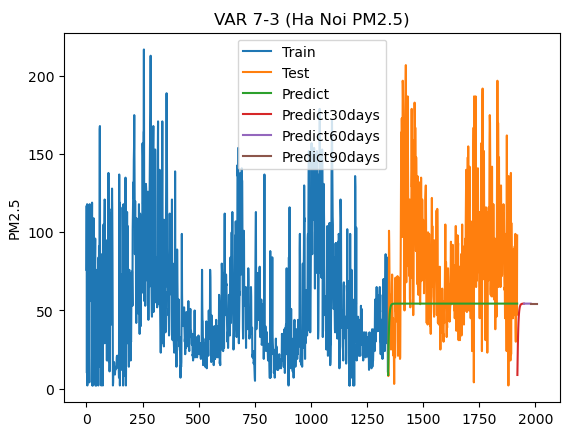
\includegraphics[width=1\textwidth]{img/final/VAR/90D/VAR_7_3_HN.png}
    \end{minipage}
    \hfill
    \begin{minipage}{0.15\textwidth}
    \centering
    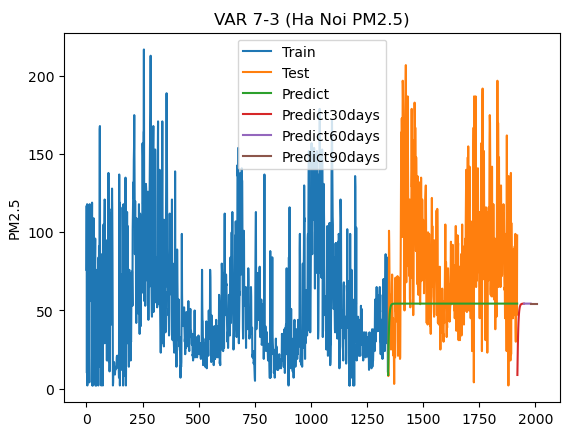
\includegraphics[width=1\textwidth]{img/final/VAR/90D/VAR_7_3_HN.png}
    \end{minipage}
    \hfill

    \begin{minipage}{0.15\textwidth}
    \centering
    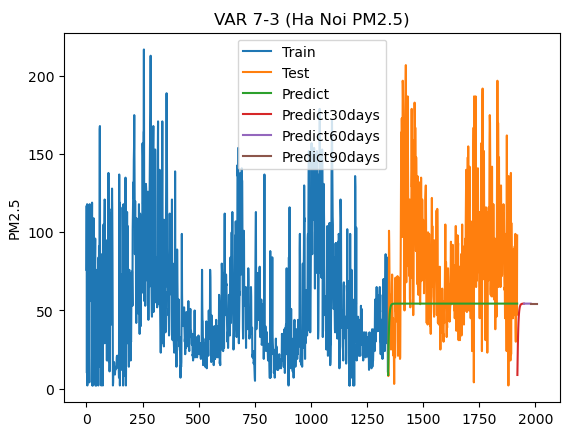
\includegraphics[width=1\textwidth]{img/final/VAR/90D/VAR_7_3_HN.png}
    \end{minipage}
    \hfill
    \begin{minipage}{0.15\textwidth}
    \centering
    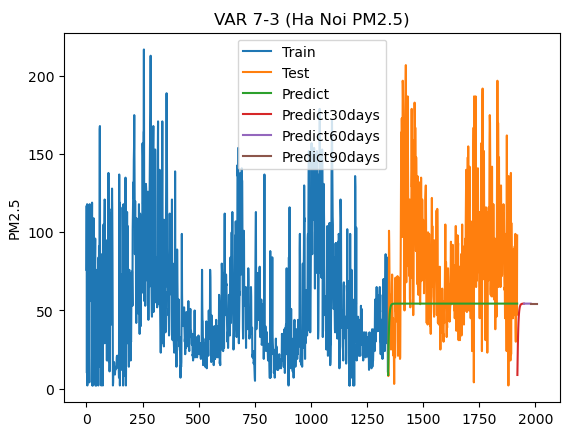
\includegraphics[width=1\textwidth]{img/final/VAR/90D/VAR_7_3_HN.png}
    \end{minipage}
    \hfill
    \begin{minipage}{0.15\textwidth}
    \centering
    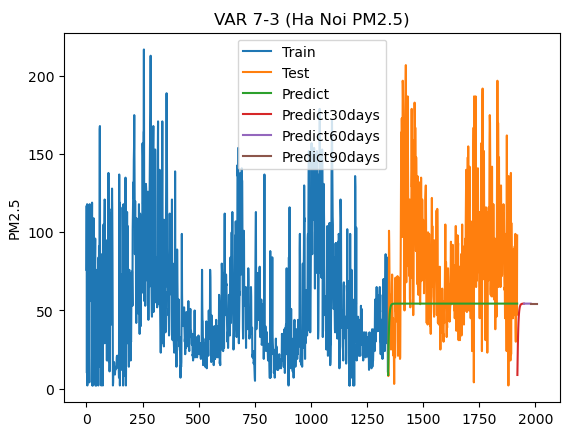
\includegraphics[width=1\textwidth]{img/final/VAR/90D/VAR_7_3_HN.png}
    \end{minipage}
    \hfill
    
    \caption{Kết quả chạy của mô hình VAR}
    \label{fig:VAR}
\end{figure}


\begin{figure}[H]
    \makebox[\textwidth][l]{1. Random Forest}

    \centering
    \begin{minipage}{0.15\textwidth}
    \centering
    \end{minipage}
    \hfill

    \begin{minipage}{0.15\textwidth}
    \centering
    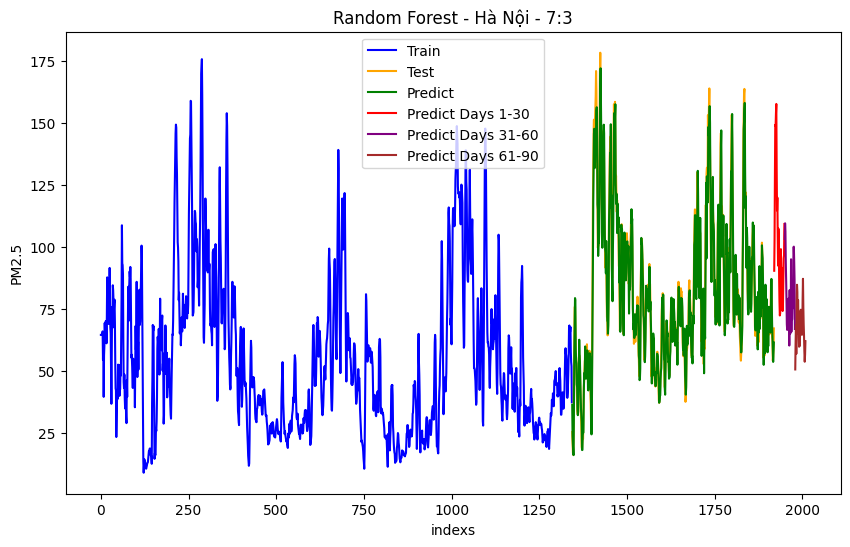
\includegraphics[width=1\textwidth]{img/final/RF/90D/RF_7_3_HN.png}
    \end{minipage}
    \hfill
    \begin{minipage}{0.15\textwidth}
    \centering
    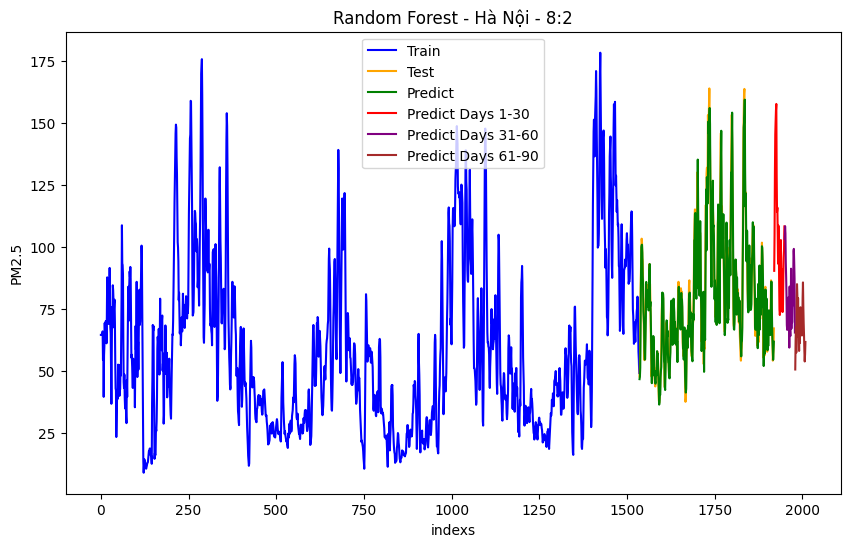
\includegraphics[width=1\textwidth]{img/final/RF/90D/RF_8_2_HN.png}
    \end{minipage}
    \hfill
    \begin{minipage}{0.15\textwidth}
    \centering
    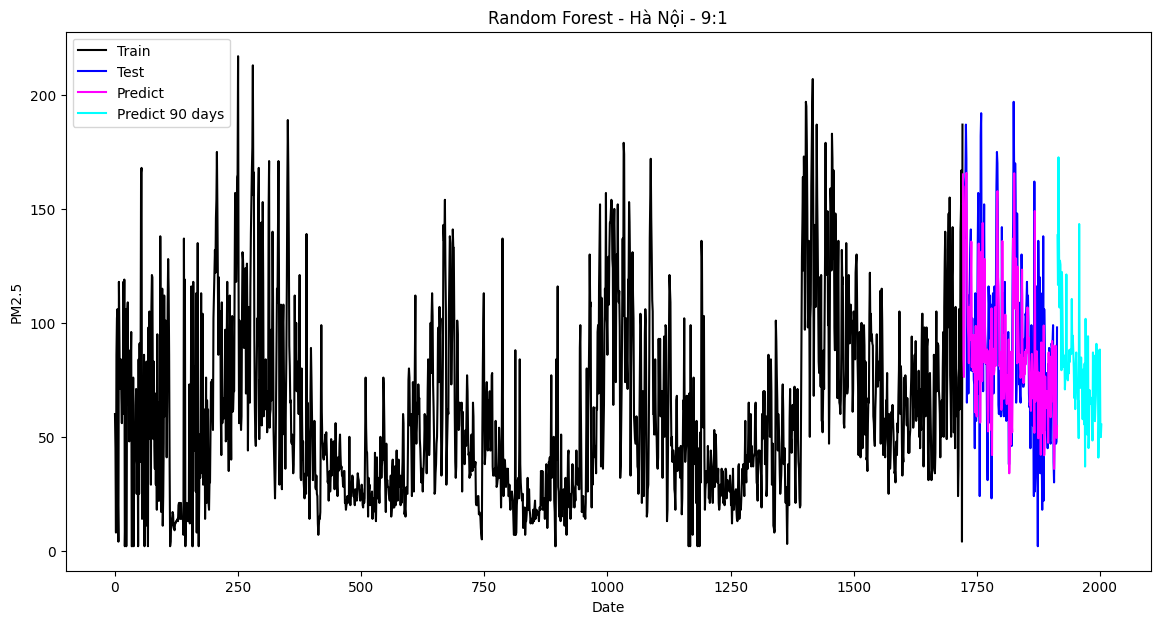
\includegraphics[width=1\textwidth]{img/final/RF/90D/RF_9_1_HN.png}
    \end{minipage}
    \hfill

    \begin{minipage}{0.15\textwidth}
    \centering
    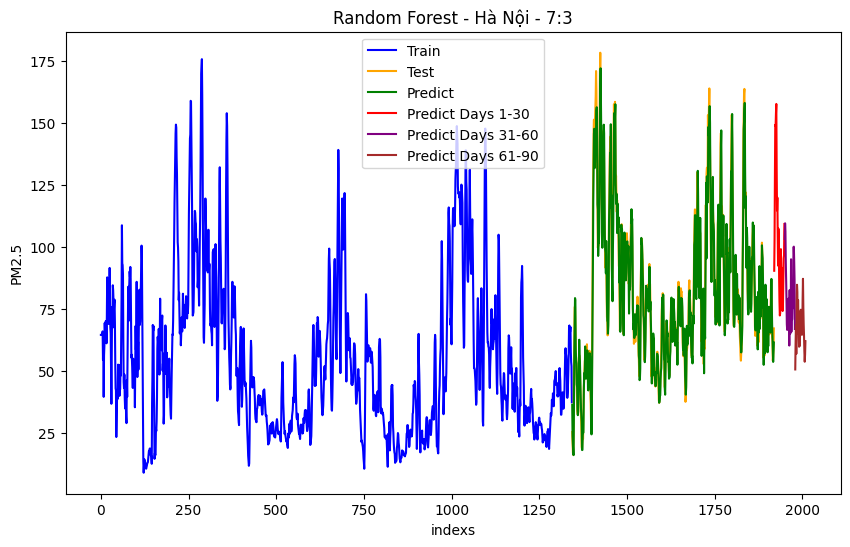
\includegraphics[width=1\textwidth]{img/final/RF/90D/RF_7_3_HN.png}
    \end{minipage}
    \hfill
    \begin{minipage}{0.15\textwidth}
    \centering
    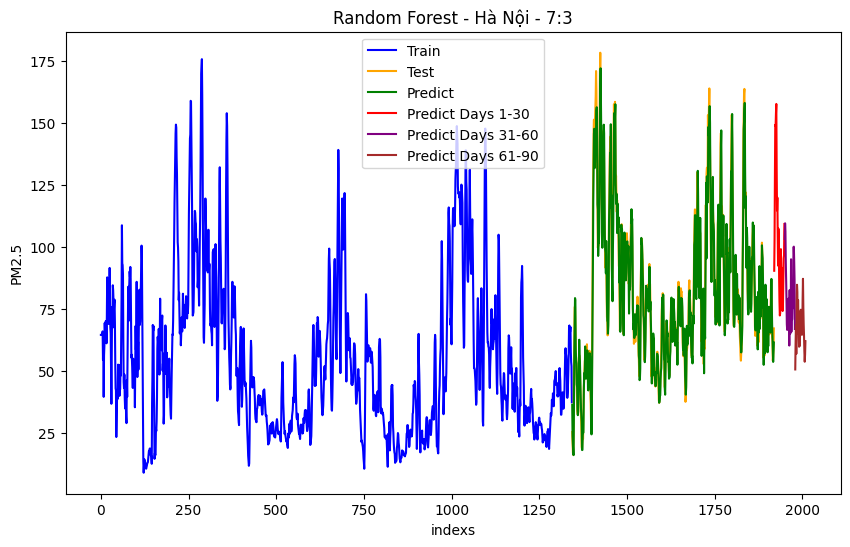
\includegraphics[width=1\textwidth]{img/final/RF/90D/RF_7_3_HN.png}
    \end{minipage}
    \hfill
    \begin{minipage}{0.15\textwidth}
    \centering
    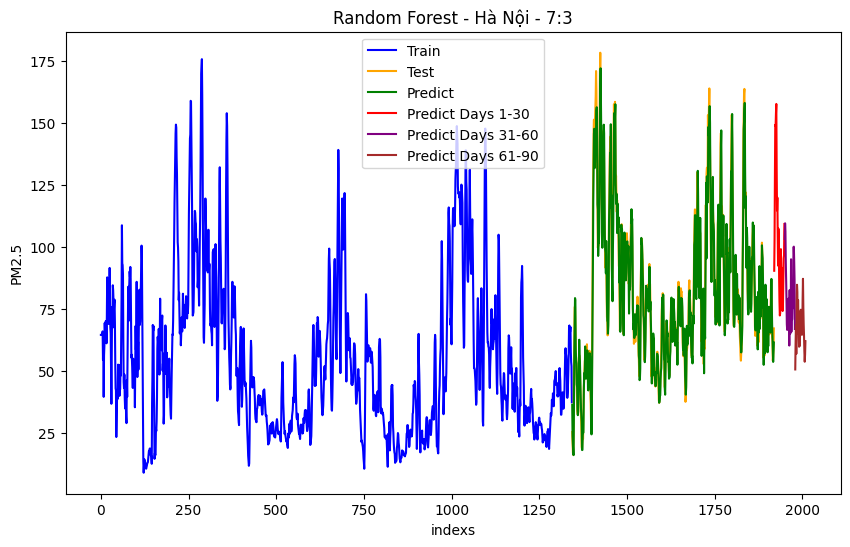
\includegraphics[width=1\textwidth]{img/final/RF/90D/RF_7_3_HN.png}
    \end{minipage}
    \hfill

    \begin{minipage}{0.15\textwidth}
    \centering
    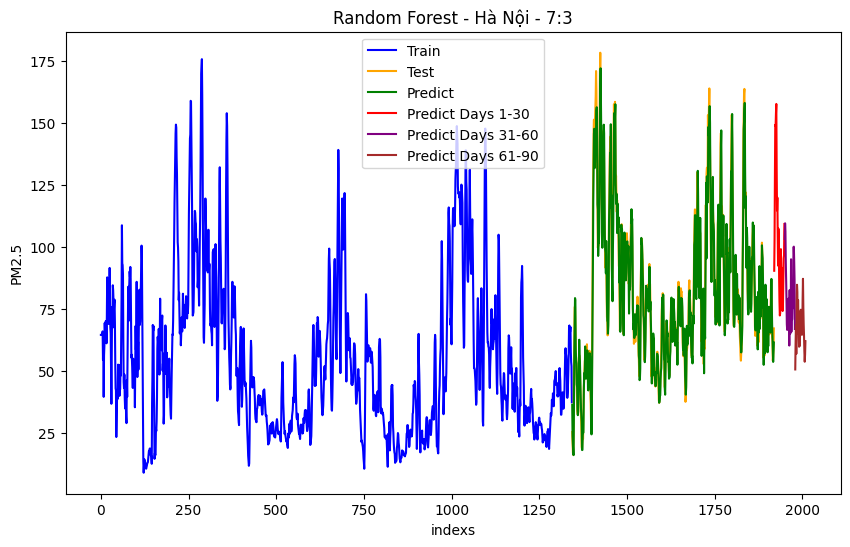
\includegraphics[width=1\textwidth]{img/final/RF/90D/RF_7_3_HN.png}
    \end{minipage}
    \hfill
    \begin{minipage}{0.15\textwidth}
    \centering
    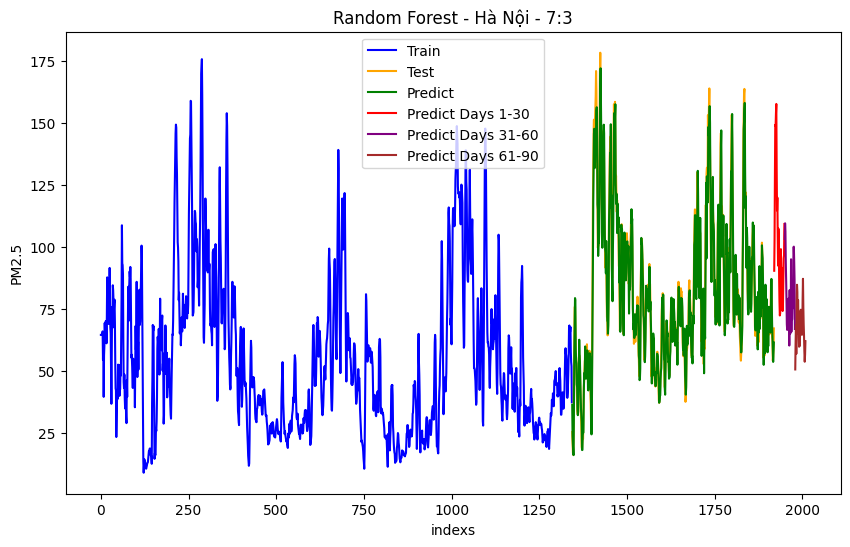
\includegraphics[width=1\textwidth]{img/final/RF/90D/RF_7_3_HN.png}
    \end{minipage}
    \hfill
    \begin{minipage}{0.15\textwidth}
    \centering
    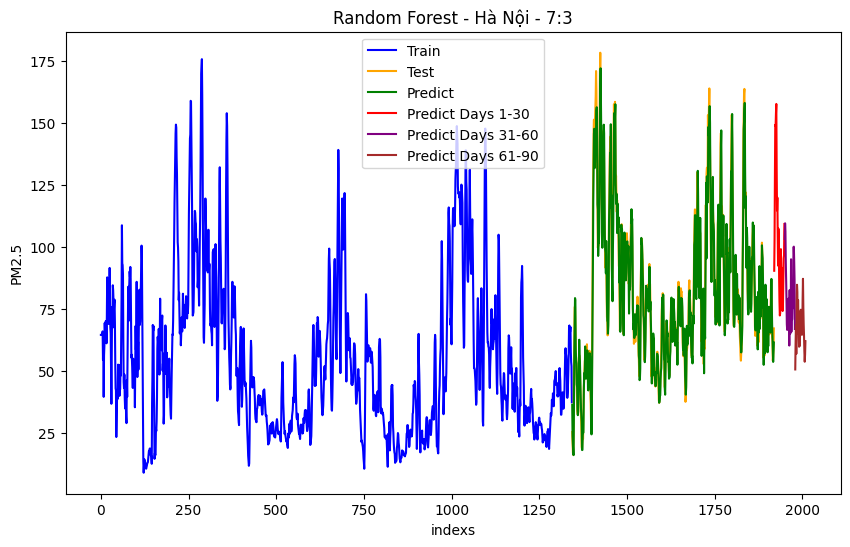
\includegraphics[width=1\textwidth]{img/final/RF/90D/RF_7_3_HN.png}
    \end{minipage}
    \hfill
    
    \caption{Kết quả chạy của mô hình Random Forest}
    \label{fig:Random_Forest}
\end{figure}


\begin{figure}[H]
    \makebox[\textwidth][l]{9. TiDE}

    \centering
    \begin{minipage}{0.15\textwidth}
    \centering
    \end{minipage}
    \hfill

    \begin{minipage}{0.15\textwidth}
    \centering
    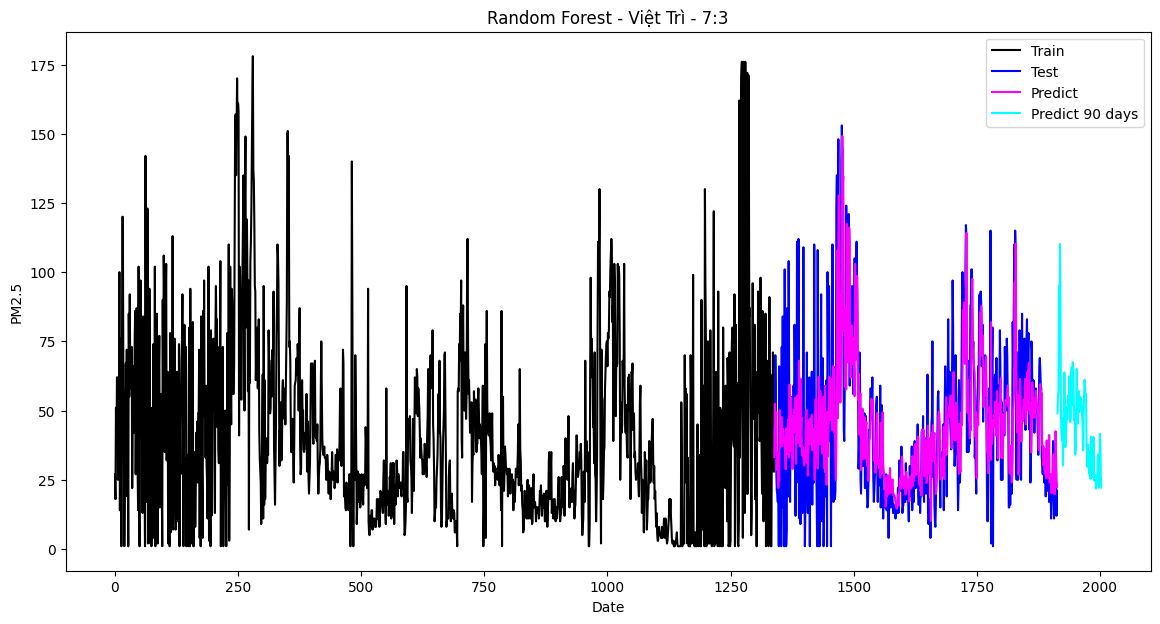
\includegraphics[width=1\textwidth]{img/final/RF/90D/RF_7_3_VT.png}
    \end{minipage}
    \hfill
    \begin{minipage}{0.15\textwidth}
    \centering
    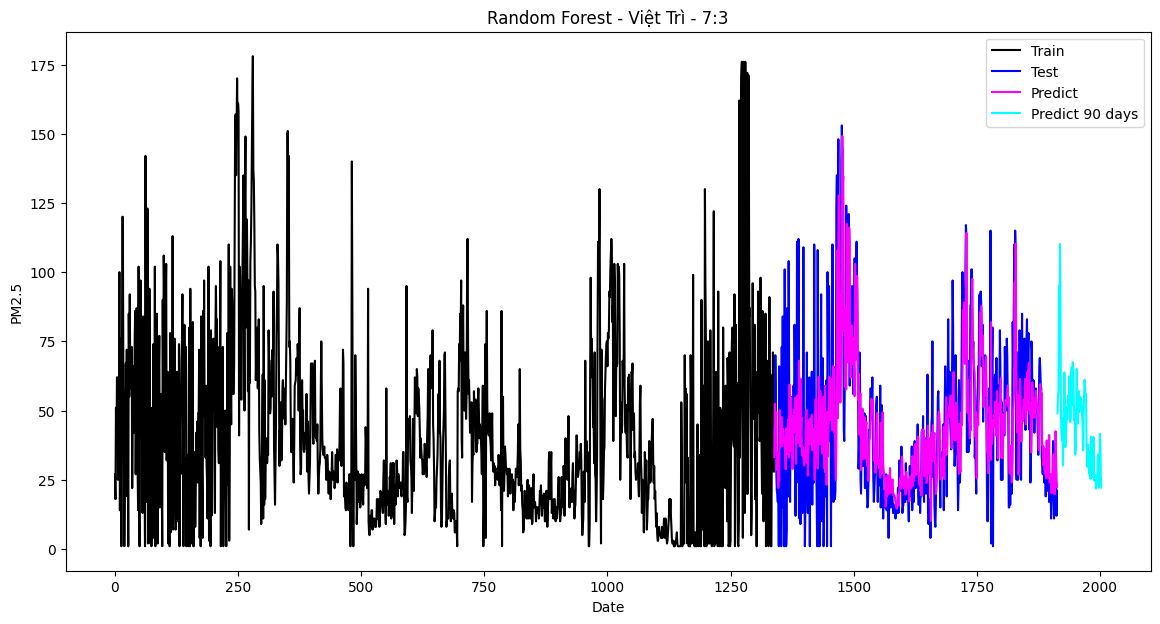
\includegraphics[width=1\textwidth]{img/final/RF/90D/RF_7_3_VT.png}
    \end{minipage}
    \hfill
    \begin{minipage}{0.15\textwidth}
    \centering
    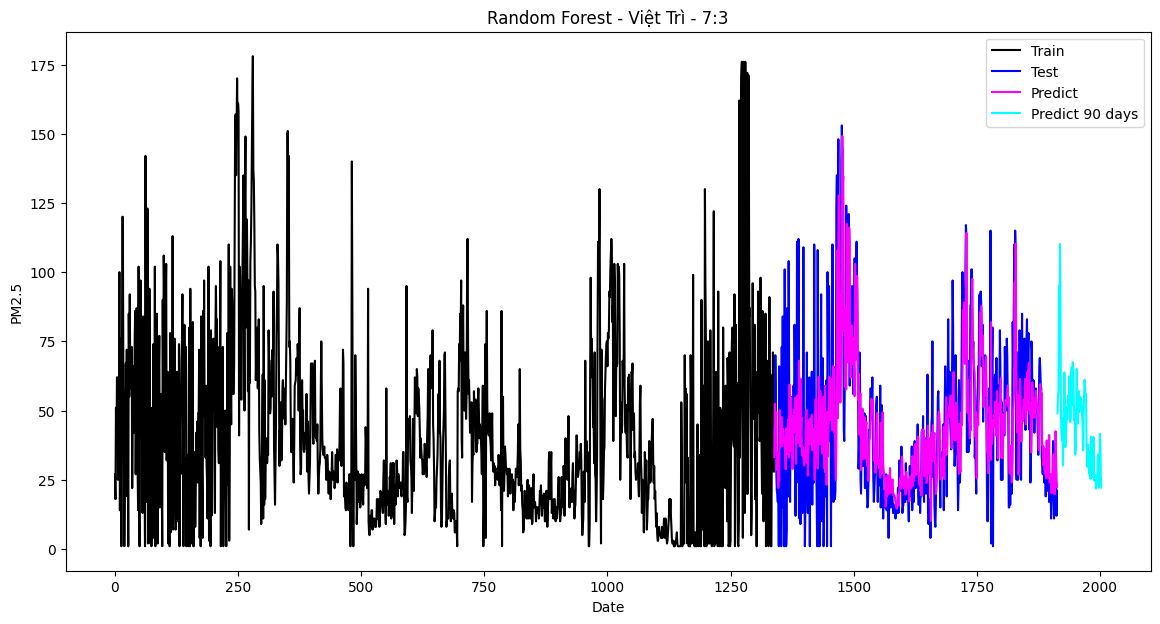
\includegraphics[width=1\textwidth]{img/final/RF/90D/RF_7_3_VT.png}
    \end{minipage}
    \hfill

    \begin{minipage}{0.15\textwidth}
    \centering
    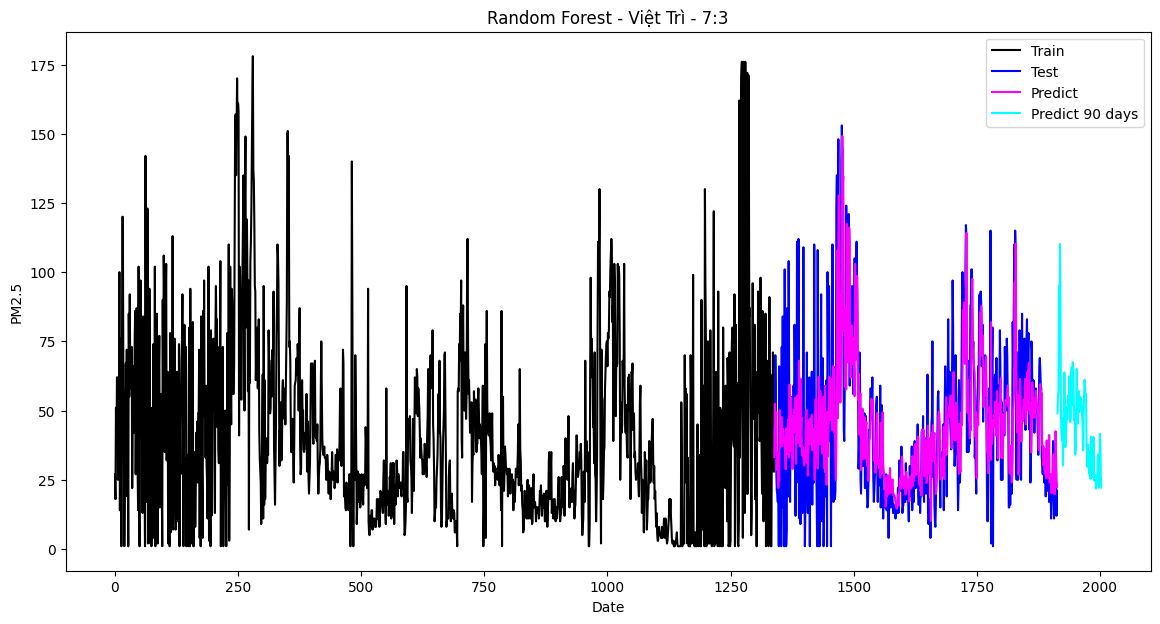
\includegraphics[width=1\textwidth]{img/final/RF/90D/RF_7_3_VT.png}
    \end{minipage}
    \hfill
    \begin{minipage}{0.15\textwidth}
    \centering
    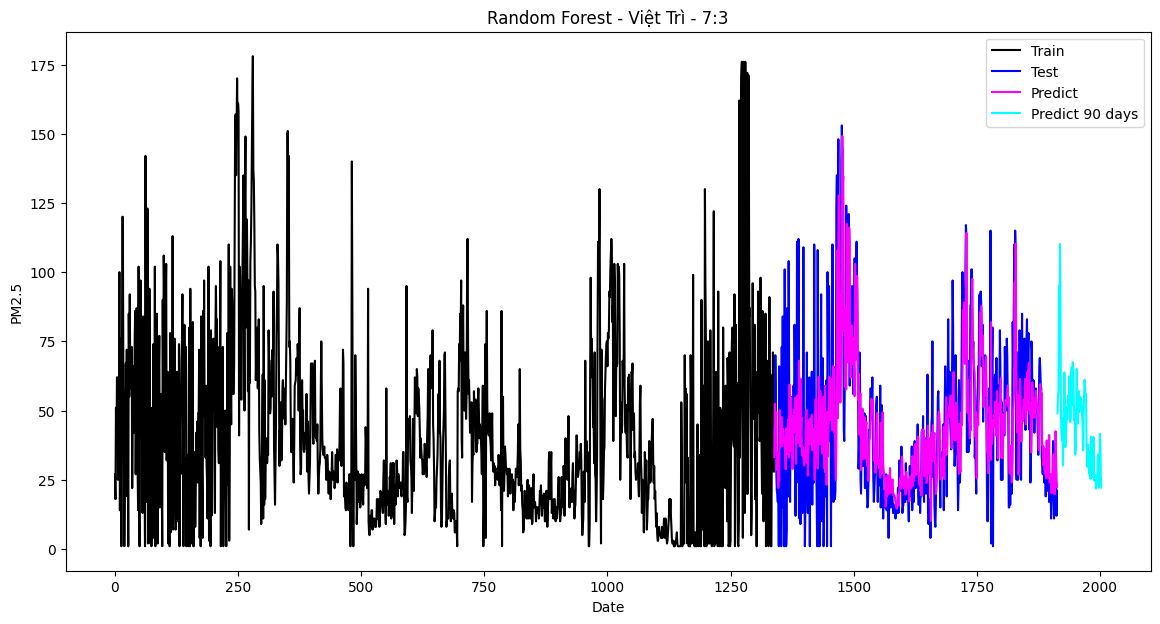
\includegraphics[width=1\textwidth]{img/final/RF/90D/RF_7_3_VT.png}
    \end{minipage}
    \hfill
    \begin{minipage}{0.15\textwidth}
    \centering
    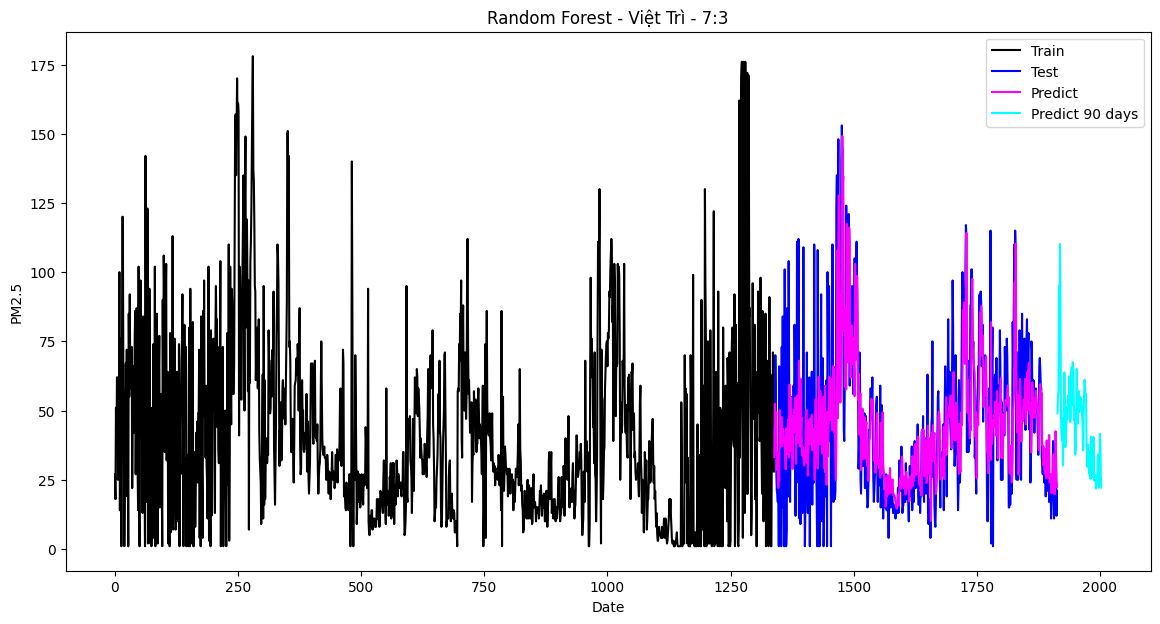
\includegraphics[width=1\textwidth]{img/final/RF/90D/RF_7_3_VT.png}
    \end{minipage}
    \hfill

    \begin{minipage}{0.15\textwidth}
    \centering
    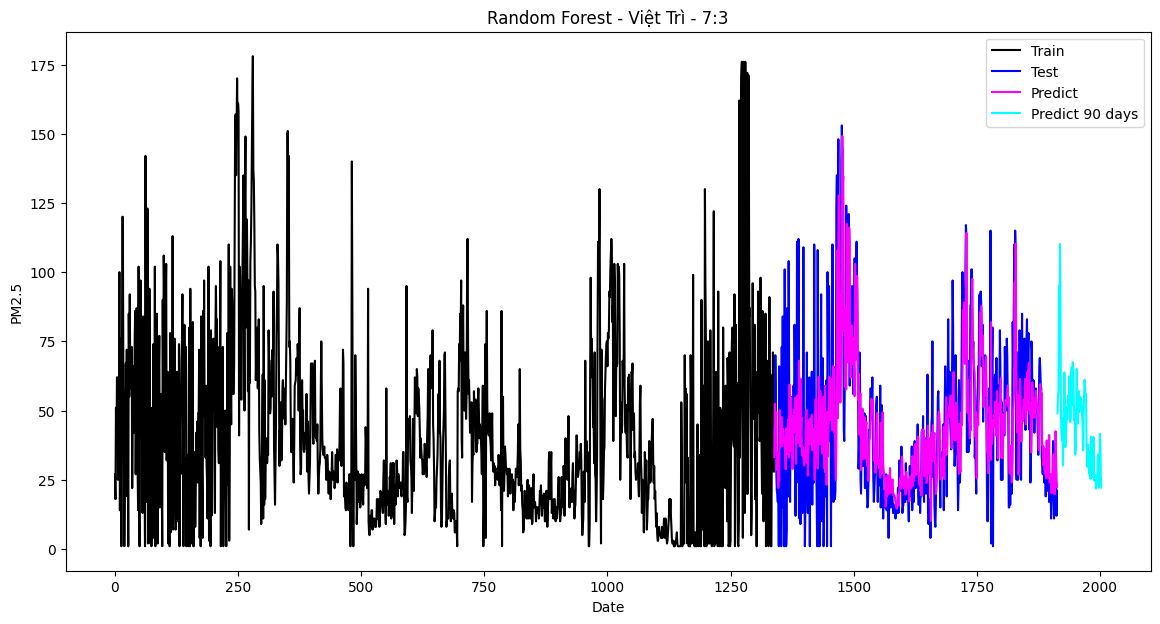
\includegraphics[width=1\textwidth]{img/final/RF/90D/RF_7_3_VT.png}
    \end{minipage}
    \hfill
    \begin{minipage}{0.15\textwidth}
    \centering
    \includegraphics[width=1\textwidth]{img/final/RF/90D/RF_7_3_VT.png}
    \end{minipage}
    \hfill
    \begin{minipage}{0.15\textwidth}
    \centering
    \includegraphics[width=1\textwidth]{img/final/RF/90D/RF_7_3_VT.png}
    \end{minipage}
    \hfill
    
    \caption{Kết quả chạy của mô hình Random Forest}
    \label{fig:Random_Forest}
\end{figure}


\begin{figure}[H]
    \makebox[\textwidth][l]{6. RNN}

    \centering
    \begin{minipage}{0.15\textwidth}
    \centering
    \end{minipage}
    \hfill

    \begin{minipage}{0.15\textwidth}
    \centering
    \includegraphics[width=1\textwidth]{img/final/RNN/90D/RNN_7_3_HN.png}
    \end{minipage}
    \hfill
    \begin{minipage}{0.15\textwidth}
    \centering
    \includegraphics[width=1\textwidth]{img/final/RNN/90D/RNN_8_2_HN.png}
    \end{minipage}
    \hfill
    \begin{minipage}{0.15\textwidth}
    \centering
    \includegraphics[width=1\textwidth]{img/final/RNN/90D/RNN_9_1_HN.png}
    \end{minipage}
    \hfill

    \begin{minipage}{0.15\textwidth}
    \centering
    \includegraphics[width=1\textwidth]{img/final/RNN/90D/RNN_7_3_HL.png}
    \end{minipage}
    \hfill
    \begin{minipage}{0.15\textwidth}
    \centering
    \includegraphics[width=1\textwidth]{img/final/RNN/90D/RNN_8_2_HL.png}
    \end{minipage}
    \hfill
    \begin{minipage}{0.15\textwidth}
    \centering
    \includegraphics[width=1\textwidth]{img/final/RNN/90D/RNN_9_1_HL.png}
    \end{minipage}
    \hfill

    \begin{minipage}{0.15\textwidth}
    \centering
    \includegraphics[width=1\textwidth]{img/final/RNN/90D/RNN_7_3_VT.png}
    \end{minipage}
    \hfill
    \begin{minipage}{0.15\textwidth}
    \centering
    \includegraphics[width=1\textwidth]{img/final/RNN/90D/RNN_8_2_VT.png}
    \end{minipage}
    \hfill
    \begin{minipage}{0.15\textwidth}
    \centering
    \includegraphics[width=1\textwidth]{img/final/RNN/90D/RNN_9_1_VT.png}
    \end{minipage}
    \hfill
    
    \caption{Kết quả chạy của mô hình RNN}
    \label{fig:RNN}
\end{figure}


\begin{figure}[H]
    \makebox[\textwidth][l]{7. GRU}

    \centering
    \begin{minipage}{0.15\textwidth}
    \centering
    \end{minipage}
    \hfill

    \begin{minipage}{0.15\textwidth}
    \centering
    \includegraphics[width=1\textwidth]{img/final/RF/90D/RF_7_3_VT.png}
    \end{minipage}
    \hfill
    \begin{minipage}{0.15\textwidth}
    \centering
    \includegraphics[width=1\textwidth]{img/final/RF/90D/RF_7_3_VT.png}
    \end{minipage}
    \hfill
    \begin{minipage}{0.15\textwidth}
    \centering
    \includegraphics[width=1\textwidth]{img/final/RF/90D/RF_7_3_VT.png}
    \end{minipage}
    \hfill

    \begin{minipage}{0.15\textwidth}
    \centering
    \includegraphics[width=1\textwidth]{img/final/RF/90D/RF_7_3_VT.png}
    \end{minipage}
    \hfill
    \begin{minipage}{0.15\textwidth}
    \centering
    \includegraphics[width=1\textwidth]{img/final/RF/90D/RF_7_3_VT.png}
    \end{minipage}
    \hfill
    \begin{minipage}{0.15\textwidth}
    \centering
    \includegraphics[width=1\textwidth]{img/final/RF/90D/RF_7_3_VT.png}
    \end{minipage}
    \hfill

    \begin{minipage}{0.15\textwidth}
    \centering
    \includegraphics[width=1\textwidth]{img/final/RF/90D/RF_7_3_VT.png}
    \end{minipage}
    \hfill
    \begin{minipage}{0.15\textwidth}
    \centering
    \includegraphics[width=1\textwidth]{img/final/RF/90D/RF_7_3_VT.png}
    \end{minipage}
    \hfill
    \begin{minipage}{0.15\textwidth}
    \centering
    \includegraphics[width=1\textwidth]{img/final/RF/90D/RF_7_3_VT.png}
    \end{minipage}
    \hfill
    
    \caption{Kết quả chạy của mô hình Random Forest}
    \label{fig:Random_Forest}
\end{figure}


\begin{figure}[H]
    \makebox[\textwidth][l]{8. LSTM}

    \centering
    \begin{minipage}{0.15\textwidth}
    \centering
    \end{minipage}
    \hfill

    \begin{minipage}{0.15\textwidth}
    \centering
    \includegraphics[width=1\textwidth]{img/final/RF/90D/RF_7_3_VT.png}
    \end{minipage}
    \hfill
    \begin{minipage}{0.15\textwidth}
    \centering
    \includegraphics[width=1\textwidth]{img/final/RF/90D/RF_7_3_VT.png}
    \end{minipage}
    \hfill
    \begin{minipage}{0.15\textwidth}
    \centering
    \includegraphics[width=1\textwidth]{img/final/RF/90D/RF_7_3_VT.png}
    \end{minipage}
    \hfill

    \begin{minipage}{0.15\textwidth}
    \centering
    \includegraphics[width=1\textwidth]{img/final/RF/90D/RF_7_3_VT.png}
    \end{minipage}
    \hfill
    \begin{minipage}{0.15\textwidth}
    \centering
    \includegraphics[width=1\textwidth]{img/final/RF/90D/RF_7_3_VT.png}
    \end{minipage}
    \hfill
    \begin{minipage}{0.15\textwidth}
    \centering
    \includegraphics[width=1\textwidth]{img/final/RF/90D/RF_7_3_VT.png}
    \end{minipage}
    \hfill

    \begin{minipage}{0.15\textwidth}
    \centering
    \includegraphics[width=1\textwidth]{img/final/RF/90D/RF_7_3_VT.png}
    \end{minipage}
    \hfill
    \begin{minipage}{0.15\textwidth}
    \centering
    \includegraphics[width=1\textwidth]{img/final/RF/90D/RF_7_3_VT.png}
    \end{minipage}
    \hfill
    \begin{minipage}{0.15\textwidth}
    \centering
    \includegraphics[width=1\textwidth]{img/final/RF/90D/RF_7_3_VT.png}
    \end{minipage}
    \hfill
    
    \caption{Kết quả chạy của mô hình Random Forest}
    \label{fig:Random_Forest}
\end{figure}

\begin{figure}[H]
    \makebox[\textwidth][l]{6. MLP}

    \centering
    \begin{minipage}{0.15\textwidth}
    \centering
    \end{minipage}
    \hfill

    \begin{minipage}{0.15\textwidth}
        \centering
        \includegraphics[width=1\textwidth]{img/final/MLP/90D/MLP_7_3_HL.png}
        \end{minipage}
        \hfill
        \begin{minipage}{0.15\textwidth}
        \centering
        \includegraphics[width=1\textwidth]{img/final/MLP/90D/MLP_7_3_HN.png}
        \end{minipage}
        \hfill
        \begin{minipage}{0.15\textwidth}
        \centering
        \includegraphics[width=1\textwidth]{img/final/MLP/90D/MLP_7_3_VT.png}
        \end{minipage}
        \hfill

    \begin{minipage}{0.15\textwidth}
        \centering
        \includegraphics[width=1\textwidth]{img/final/MLP/90D/MLP_8_2_HL.png}
        \end{minipage}
        \hfill
        \begin{minipage}{0.15\textwidth}
        \centering
        \includegraphics[width=1\textwidth]{img/final/MLP/90D/MLP_8_2_HN.png}
        \end{minipage}
        \hfill
        \begin{minipage}{0.15\textwidth}
        \centering
        \includegraphics[width=1\textwidth]{img/final/MLP/90D/MLP_8_2_VT.png}
        \end{minipage}
        \hfill

    \begin{minipage}{0.15\textwidth}
        \centering
        \includegraphics[width=1\textwidth]{img/final/MLP/90D/MLP_9_1_HL.png}
        \end{minipage}
        \hfill
        \begin{minipage}{0.15\textwidth}
        \centering
        \includegraphics[width=1\textwidth]{img/final/MLP/90D/MLP_9_1_HN.png}
        \end{minipage}
        \hfill
        \begin{minipage}{0.15\textwidth}
        \centering
        \includegraphics[width=1\textwidth]{img/final/MLP/90D/MLP_9_1_VT.png}
        \end{minipage}
        \hfill
    
    \caption{Kết quả dự báo của mô hình MLP}
    \label{fig:MLP}
    
\end{figure}15:48/-strong/-heart:>:o:-((:-hXem trước khi gửiThả Files vào đây để xem lại trước khi gửi
\begin{figure}[H]
    \makebox[\textwidth][l]{10. Autoformer}

    \centering
    \begin{minipage}{0.15\textwidth}
    \centering
    \end{minipage}
    \hfill

    \begin{minipage}{0.15\textwidth}
        \centering
        \includegraphics[width=1\textwidth]{img/final/Autoformer/90D/Autoformer_7_3_HL.png}
        \end{minipage}
        \hfill
        \begin{minipage}{0.15\textwidth}
        \centering
        \includegraphics[width=1\textwidth]{img/final/Autoformer/90D/Autoformer_7_3_HN.png}
        \end{minipage}
        \hfill
        \begin{minipage}{0.15\textwidth}
        \centering
        \includegraphics[width=1\textwidth]{img/final/Autoformer/90D/Autoformer_7_3_VT.png}
        \end{minipage}
        \hfill

    \begin{minipage}{0.15\textwidth}
        \centering
        \includegraphics[width=1\textwidth]{img/final/Autoformer/90D/Autoformer_8_2_HL.png}
        \end{minipage}
        \hfill
        \begin{minipage}{0.15\textwidth}
        \centering
        \includegraphics[width=1\textwidth]{img/final/Autoformer/90D/Autoformer_8_2_HN.png}
        \end{minipage}
        \hfill
        \begin{minipage}{0.15\textwidth}
        \centering
        \includegraphics[width=1\textwidth]{img/final/Autoformer/90D/Autoformer_8_2_VT.png}
        \end{minipage}
        \hfill

    \begin{minipage}{0.15\textwidth}
        \centering
        \includegraphics[width=1\textwidth]{img/final/Autoformer/90D/Autoformer_8_2_HL.png}
        \end{minipage}
        \hfill
        \begin{minipage}{0.15\textwidth}
        \centering
        \includegraphics[width=1\textwidth]{img/final/Autoformer/90D/Autoformer_8_2_HN.png}
        \end{minipage}
        \hfill
        \begin{minipage}{0.15\textwidth}
        \centering
        \includegraphics[width=1\textwidth]{img/final/Autoformer/90D/Autoformer_8_2_VT.png}
        \end{minipage}
        \hfill
    
    \caption{Kết quả dự báo của mô hình Autoformer}
    \label{fig:Autoformer}
\end{figure}

\subsection{Đánh giá}
\section{\textcolor{brown}{Kết luận}}
Thông qua các cuộc thử nghiệm ở cả 10 mô hình...


\begin{thebibliography}{00}
    \bibitem{b1}
    E. Marinov, D. Petrova-Antonova, and S. Malinov,
    ``Time Series Forecasting of Air Quality: A Case Study of Sofia City,''
    \textit{Atmosphere}, vol. 13, p. 788, 2022. [Online]. Available:https://www.mdpi.com/2073-4433/13/5/788
    \bibitem{b2} K. N. Sh, I. Irfani, and U. Mukhaiyar,
    ``Predicting Air Pollution Levels in Jakarta Using Vector Autoregressive Analysis,''
    \textit{Proceedings of the 5th International Conference on Statistics, Mathematics, Teaching, and Research 2023 (ICSMTR 2023)}, pp. 14-22, Atlantis Press, 2023. [Online].
    Available:https://doi.org/10.2991/978-94-6463-332-0\string_3
    \bibitem{b3}
    K. H. Waseem, H. Mushtaq, F. Abid, A. M. Abu-Mahfouz, A. Shaikh, M. Turan, and J. Rasheed,
    ``Forecasting of Air Quality Using an Optimized Recurrent Neural Network,''
    \textit{Processes}, vol. 10, no. 10, p. 2117, 2022. [Online].
    Available: https://doi.org/10.3390/pr1010211
    \bibitem{b4}
    Citation: Esager, M.W.M.; Ünlü, K.D.
    ``Forecasting Air Quality in Tripoli: An Evaluation of Deep Learning Models for Hourly PM2.5 Surface Mass Concentrations.
    \textit {Atmosphere} 2023, 14, 478. [Online].
    Available: https://doi.org/10.3390/atmos14030478
    \bibitem{b5}
    A. Das, W. Kong, A. Leach, S. Mathur, R. Sen, and R. Yu,
    ``Long-term Forecasting with TiDE: Time-series Dense Encoder,''
    \textit{arXiv:2304.08424 [stat.ML]}, April 2023.
    [Online]. Available: https://doi.org/10.48550/arXiv.2304.08424
    \bibitem{b6}
    B. T. Ong, K. Sugiura, and K. Zettsu,
    ``Dynamically pre-trained deep recurrent neural networks using environmental monitoring data for predicting PM2.5,''
    \textit{Neural Comput Appl}, vol. 27, no. 6, pp. 1553–1566, 2016.
    [Online]. Available: https://doi.org/10.1007/s00521-015-1955-3
    \bibitem{b7}
    Y. B. Lim, I. Aliyu, and C. G. Lim,
    ``Air pollution matter prediction using recurrent neural networks with sequential data,''
    In: \textit{Proceedings of the 2019 3rd International Conference on Intelligent Systems, Metaheuristics \& Swarm Intelligence. ISMSI 2019}, pp. 40–44, Association for Computing Machinery, New York, NY, USA, 2019.
    [Online]. Available: https://doi.org/10.1145/3325773.3325788
    \bibitem{b8}
    H. Wu, J. Xu, J. Wang, \& M. Long,
    ``Autoformer: Decomposition Transformers with Auto-Correlation for Long-Term Series Forecasting,''
    2021.
    
    \end{thebibliography}
    \vspace{12pt}
    
    
\end{document}